\documentclass[11pt,a4paper]{article}
\usepackage[utf8]{inputenc}
\usepackage[T1]{fontenc}
\usepackage{lmodern}
\usepackage[margin=2.2cm]{geometry}
\usepackage{graphicx,float,booktabs,longtable,array,amsmath,amssymb,xcolor,listings,caption,hyperref,newunicodechar,calc,etoolbox}
\usepackage{enumitem,textcomp}
\setlist{nosep}
\hypersetup{colorlinks=true,linkcolor=black,urlcolor=black,citecolor=black}
\captionsetup{font={small,it},labelfont={bf,it},textfont={color=black!70}}
\providecommand{\tightlist}{\setlength{\itemsep}{0pt}\setlength{\parskip}{0pt}}
\lstset{basicstyle=\ttfamily\footnotesize,breaklines=true,frame=single,rulecolor=\color{black!40},backgroundcolor=\color{black!4},columns=fullflexible,keepspaces=true}
\setlength{\parindent}{0pt}\setlength{\parskip}{5pt}
\newunicodechar{ω}{\ensuremath{\omega}}
\newunicodechar{α}{\ensuremath{\alpha}}
\newunicodechar{±}{\ensuremath{\pm}}
\newunicodechar{²}{\textsuperscript{2}}
\newunicodechar{ζ}{\ensuremath{\zeta}}
\newunicodechar{θ}{\ensuremath{\theta}}
\newunicodechar{φ}{\ensuremath{\phi}}
\newunicodechar{≈}{\ensuremath{\approx}}
\newunicodechar{√}{\ensuremath{\surd}}
\newunicodechar{Θ}{\ensuremath{\Theta}}
\newunicodechar{π}{\ensuremath{\pi}}
\newunicodechar{ŷ}{\ensuremath{\hat{y}}}
\newunicodechar{½}{\ensuremath{\tfrac12}}
\newunicodechar{∠}{\ensuremath{\angle}}
\newunicodechar{⁴}{\textsuperscript{4}}
\newunicodechar{→}{\ensuremath{\rightarrow}}
\newunicodechar{⁻}{\textsuperscript{\textminus}}
\newunicodechar{¹}{\textsuperscript{1}}
%UNI
\begin{document}
\begin{titlepage}\centering
\vspace*{3cm}
{\LARGE\bfseries ES 245: Control Systems\\[4pt] Course Project, Part 2\par}
\vspace{0.8cm}
{\large System Identification, Frequency Domain Analysis and\\ Lead / Lead-Lag Compensation of the Car on Beam (Setup 5)\par}
\vspace{1.5cm}
Dhvani Shah (24110325)\\ Sejal Sharbidre (24110322)\\ Prachi Jindal (24110264)\par
\vspace{1cm}
Department of Mechanical Engineering\\ Indian Institute of Technology Gandhinagar\\ Fall 2026\par
\vspace{1.5cm}
\begin{minipage}{0.85\linewidth}
\textbf{Summary.} We characterised our car on beam setup with four chirp experiments and identified its transfer function, $G(s) = 2.591/(s^2 + 0.4789\,s + 0.002551)$ cm/deg, with a 60.6\,\% fit. Root locus, Nyquist and Bode analysis showed a stable but poorly damped loop (phase margin 16.9 deg, 62\,\% overshoot, 12 s settling). A lead compensator with a prefilter raised the phase margin to 61.7 deg and met both specifications in simulation (0\,\% overshoot, 2.1 s settling with the measured delay). On the hardware the lead moved the car to the target in about 2 s, but wheel friction left a 1.7 to 4.8 cm offset. Adding a lag stage (lead-lag) removed that offset (final error 0.09 to 0.43 cm). Where friction held the car, a light push by hand freed it, and the controller brought it back to the target within about 1 to 2 s.
\end{minipage}
\end{titlepage}
\tableofcontents
\newpage
\hypertarget{setup-units-and-the-part-1-model}{%
\section{Setup, units and the Part 1
model}\label{setup-units-and-the-part-1-model}}

A servo rotates a horn of radius d = 5 cm. A link of length l = 11 cm
joins the horn to the beam at L = 25 cm from the beam pivot, so a servo
rotation θ tilts the beam by about α = (d/L)θ. A toy car rolls on the
beam and an HC-SR04 ultrasonic sensor at one end measures its distance
a. An Arduino Mega reads the sensor and drives the servo.

\begin{figure}[H]\centering
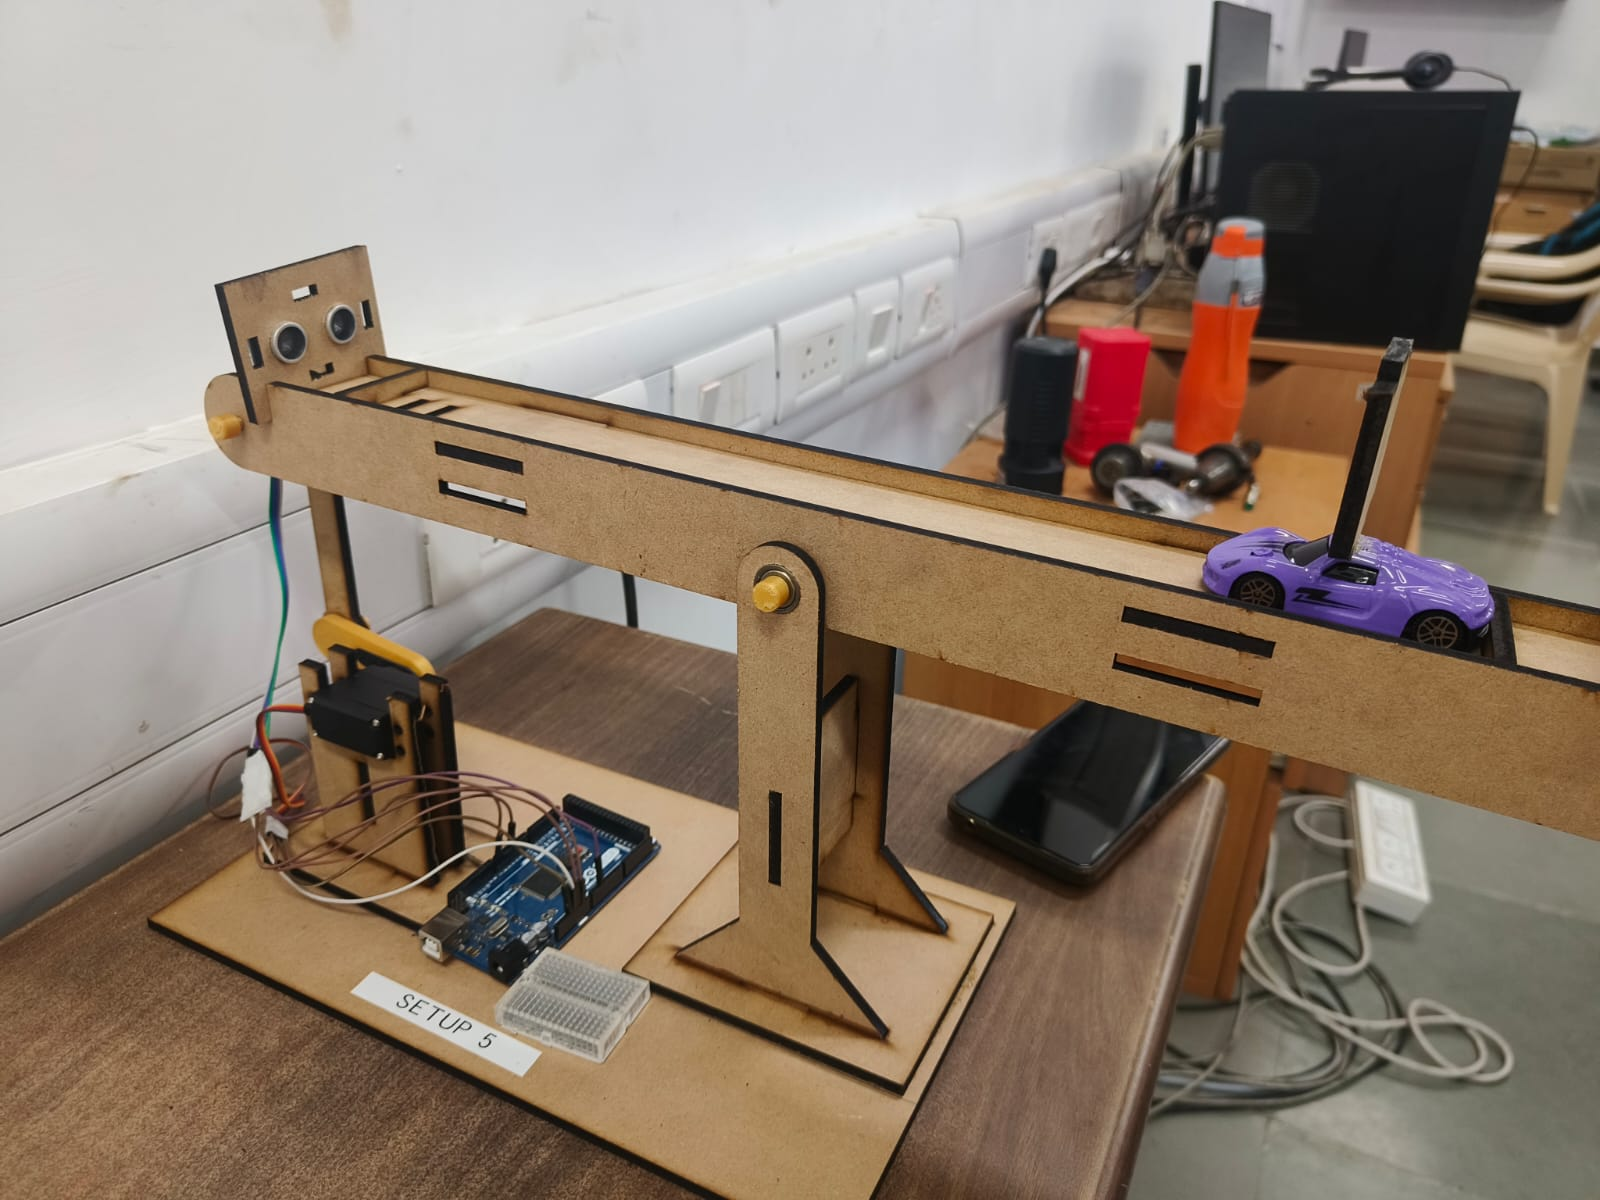
\includegraphics[width=0.6\linewidth]{figures/fig01.jpg}
\caption{Lab Setup 5: servo and four bar link (left), beam on its centre pivot,
toy car with target plate, ultrasonic sensor at the left end and the
Arduino Mega on the base.}\label{fig:1}
\end{figure}

All Part 2 work uses the units the Arduino uses, so gains can be typed
straight into the code:

\begin{itemize}
\tightlist
\item
  input u (or θ): servo angle measured from its centre, in degrees
\item
  output a: car position from the sensor, in centimetres
\end{itemize}

Part 1 derived the plant from the Lagrangian of the rolling car. For
small angles and negligible wheel inertia the car accelerates as a = g
α, which gives

\texttt{G\_P1(s)\ =\ A(s)/Θ(s)\ =\ (g\ d\ /\ L)\ /\ s²\ =\ 1.962\ m/(rad\ s²)\ /\ s²\ =\ 3.424\ cm/(deg\ s²)\ /\ s²}

(conversion: 1.962 m/rad x 100 cm/m / 57.3 deg/rad = 3.424). This double
integrator is the reference we compare the measured model against. Part
1 also measured two hardware facts used again here: a static friction
band of about 7 to 9 deg of servo angle in which the car does not move,
and about 70 ms of servo plus sensor delay.

\hypertarget{task-5-system-characterisation}{%
\section{Task 5: System
characterisation}\label{task-5-system-characterisation}}

\emph{What the task asks: excite the setup with a chirp, record the
response, find the transfer function with n4sid, and analyse its Bode
plot.}

\hypertarget{the-chirp-signal}{%
\subsection{The chirp signal}\label{the-chirp-signal}}

A chirp is a sine whose frequency rises with time, so one 20 s
experiment tests many frequencies. The provided sketch commands

\texttt{θ(t)\ =\ θc\ +\ A\ sin(\ 2π\ (\ f0\ t\ +\ ½\ k\ t²\ )\ ),\ \ \ \ \ \ k\ =\ (f1\ -\ f0)/T,\ \ \ \ \ \ f(t)\ =\ f0\ +\ k\ t}

with servo centre θc = 89 deg, start frequency f0 = 0.1 Hz and length T
= 20 s. The Arduino printed time, servo command and distance about every
20 ms. We ran four trials, changing the amplitude A and the end
frequency f1.

\textbf{Table 1: The four chirp trials}

\begin{longtable}[]{@{}
  >{\raggedright\arraybackslash}p{(\columnwidth - 10\tabcolsep) * \real{0.1667}}
  >{\raggedright\arraybackslash}p{(\columnwidth - 10\tabcolsep) * \real{0.1667}}
  >{\raggedright\arraybackslash}p{(\columnwidth - 10\tabcolsep) * \real{0.1667}}
  >{\raggedright\arraybackslash}p{(\columnwidth - 10\tabcolsep) * \real{0.1667}}
  >{\raggedright\arraybackslash}p{(\columnwidth - 10\tabcolsep) * \real{0.1667}}
  >{\raggedright\arraybackslash}p{(\columnwidth - 10\tabcolsep) * \real{0.1667}}@{}}
\toprule\noalign{}
\begin{minipage}[b]{\linewidth}\raggedright
Trial
\end{minipage} & \begin{minipage}[b]{\linewidth}\raggedright
File
\end{minipage} & \begin{minipage}[b]{\linewidth}\raggedright
A
\end{minipage} & \begin{minipage}[b]{\linewidth}\raggedright
f1
\end{minipage} & \begin{minipage}[b]{\linewidth}\raggedright
Frequencies kept (t = 10 to 20 s)
\end{minipage} & \begin{minipage}[b]{\linewidth}\raggedright
What the car did
\end{minipage} \\
\midrule\noalign{}
\endhead
\bottomrule\noalign{}
\endlastfoot
1 & G21A20f11 & 20 deg & 1.0 Hz & 0.55 to 1.0 Hz (3.5 to 6.3 rad/s) &
moved about +/-4 cm, never hit an end \\
2 & G21A25f11 & 25 deg & 1.0 Hz & 0.55 to 1.0 Hz & pressed against the
sensor end from 11.5 to 14.8 s \\
3 & G21A20f12.5 & 20 deg & 2.5 Hz & 1.3 to 2.5 Hz (8 to 16 rad/s) &
moved under +/-1 cm \\
4 & G21A25f11.5 & 25 deg & 1.5 Hz & 0.8 to 1.5 Hz (5 to 9.4 rad/s) &
moved about +/-1 to 2 cm \\
\end{longtable}

\begin{figure}[H]\centering
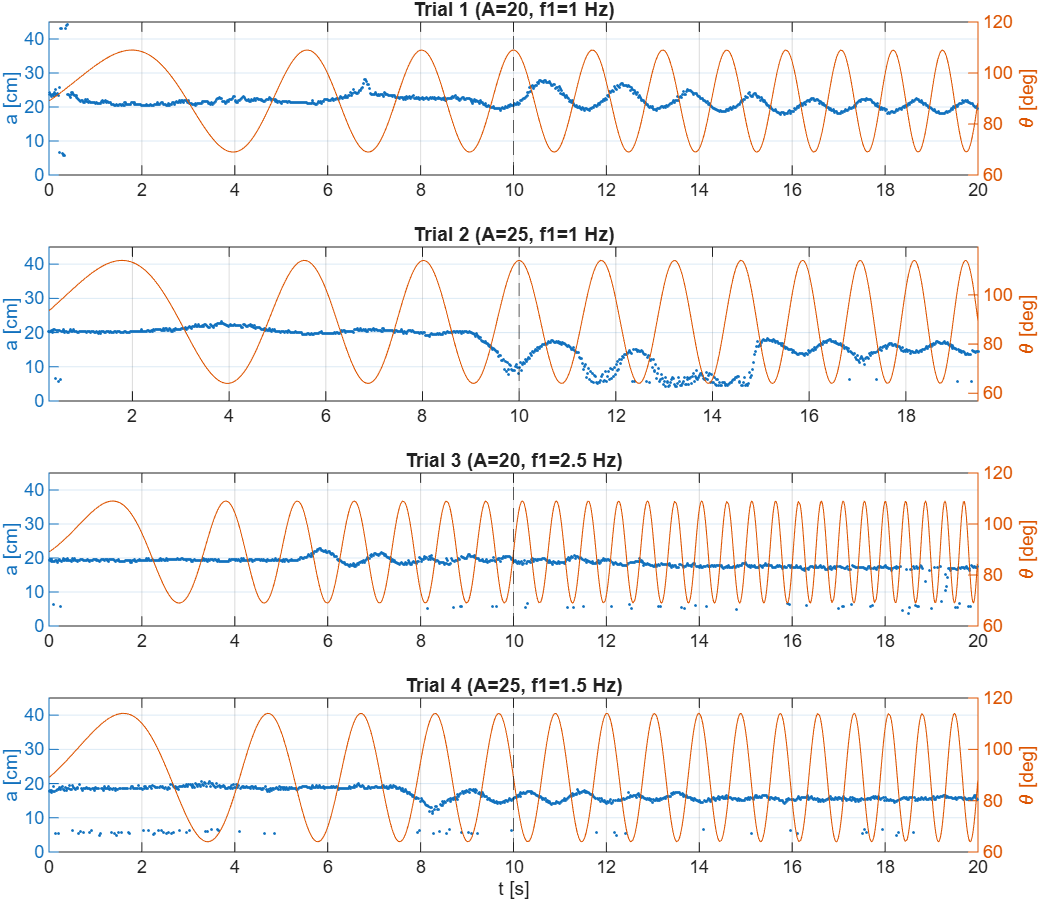
\includegraphics[width=0.92\linewidth]{figures/fig02.png}
\caption{Raw logs. Blue dots: car position. Orange: servo command. The dashed
line marks t = 10 s; data before it was removed.}\label{fig:2}
\end{figure}

\hypertarget{cleaning-the-data}{%
\subsection{Cleaning the data}\label{cleaning-the-data}}

\begin{enumerate}
\def\labelenumi{\arabic{enumi}.}
\tightlist
\item
  Removed the first 10 s (10000 ms) of every file. During the slow start
  of the sweep the car barely moved (the swing stayed inside the
  friction band for long stretches), so that part carries little
  information.
\item
  Removed readings of -1. The sensor code returns -1 when no echo
  arrives within 30 ms.
\item
  Replaced ghost echoes. The HC-SR04 sometimes reports about 5 cm for a
  single sample while the car is at 15 to 20 cm. Any sample more than
  2.5 cm away from the median of its 7 neighbours was replaced by that
  median (0, 8, 40 and 15 samples in trials 1 to 4).
\item
  Resampled onto an even 20 ms grid with linear interpolation.
  Identification tools assume a constant sample time and the Arduino
  timing jittered between 17 and 22 ms. This left 499, 505, 473 and 499
  samples.
\item
  Subtracted the servo centre (89 deg) from the input and the mean
  position from the output, so the model describes small motion about
  the operating point.
\end{enumerate}

\hypertarget{how-we-obtained-the-transfer-function}{%
\subsection{How we obtained the transfer
function}\label{how-we-obtained-the-transfer-function}}

Trial 1 was used for estimation. It has the largest motion (about ten
times the +/-0.25 cm sensor noise) and the car never reached an end.
Trials 2 to 4 were kept aside to check the model. All identification was
done in MATLAB (System Identification Toolbox) with the script
ES245\_Part2\_Solve.m.

\textbf{Step 1: n4sid, as the brief asks.}

n4sid is a subspace method. It stacks past and future inputs and outputs
into large block matrices, uses a projection and a singular value
decomposition to estimate the internal states, and then finds the state
space matrices A, B, C and D by least squares. We asked for a second
order continuous time model (the physics has two states: position and
velocity):

\begin{lstlisting}
opt    = n4sidOptions('Focus','simulation','InitialState','estimate');
sys_n4 = n4sid(dEst, 2, 'Ts', 0, opt);
\end{lstlisting}

\texttt{G\_n4sid(s)\ =\ (-3184\ s\ -\ 7721)\ /\ (s²\ +\ 1416\ s\ +\ 3623)}

Its poles are at -2.6 and -1413.5 rad/s, and its fit to the measured
data is 0 \% or less (Figure 3). The pole at -1413 rad/s is far above
157 rad/s, the highest frequency that 20 ms sampling can even represent,
and the zero has no physical source. With only a narrow band of
excitation (3.5 to 6.3 rad/s) and noisy data, the unconstrained method
fitted the noise. We therefore kept the same model order but added what
we know about the physics.

\textbf{Step 2: structured estimate with the same order.}

A tilted beam produces an acceleration of the car, so the transfer
function from servo angle to position must have two poles and no zero.
tfest fits exactly that structure by minimising the simulation error
between the model output and the measured position, while also
estimating the initial position and velocity:

\begin{lstlisting}
init   = idtf(3, [1 0.5 0.5]);              % neutral starting guess
optT   = tfestOptions('InitialCondition','estimate','EnforceStability',false);
sys_id = tfest(dEst, init, optT);           % 2 poles, 0 zeros
\end{lstlisting}

(Starting from the Part 1 model 3.424/s² left the estimate stuck at its
starting point, so a neutral starting guess was used. MATLAB reported
``Estimated using TFEST''.) The result is the model used in the rest of
this report:

\texttt{G(s)\ =\ A(s)/Θ(s)\ =\ 2.591\ /\ (s²\ +\ 0.4789\ s\ +\ 0.002551)\ \ \ {[}cm/deg{]}}

Poles: s = -0.4735 and s = -0.0054 rad/s. The fit measure MATLAB uses is

\texttt{Fit\ =\ 100\ (\ 1\ -\ \textbar{}\textbar{}y\ -\ ŷ\textbar{}\textbar{}\ /\ \textbar{}\textbar{}y\ -\ mean(y)\textbar{}\textbar{}\ )\ \%\ \ =\ \ 60.6\ \%}

where y is the measured and ŷ the simulated position. 100 \% would be a
perfect match; 0 \% means the model is no better than a flat line at the
mean.

\begin{figure}[H]\centering
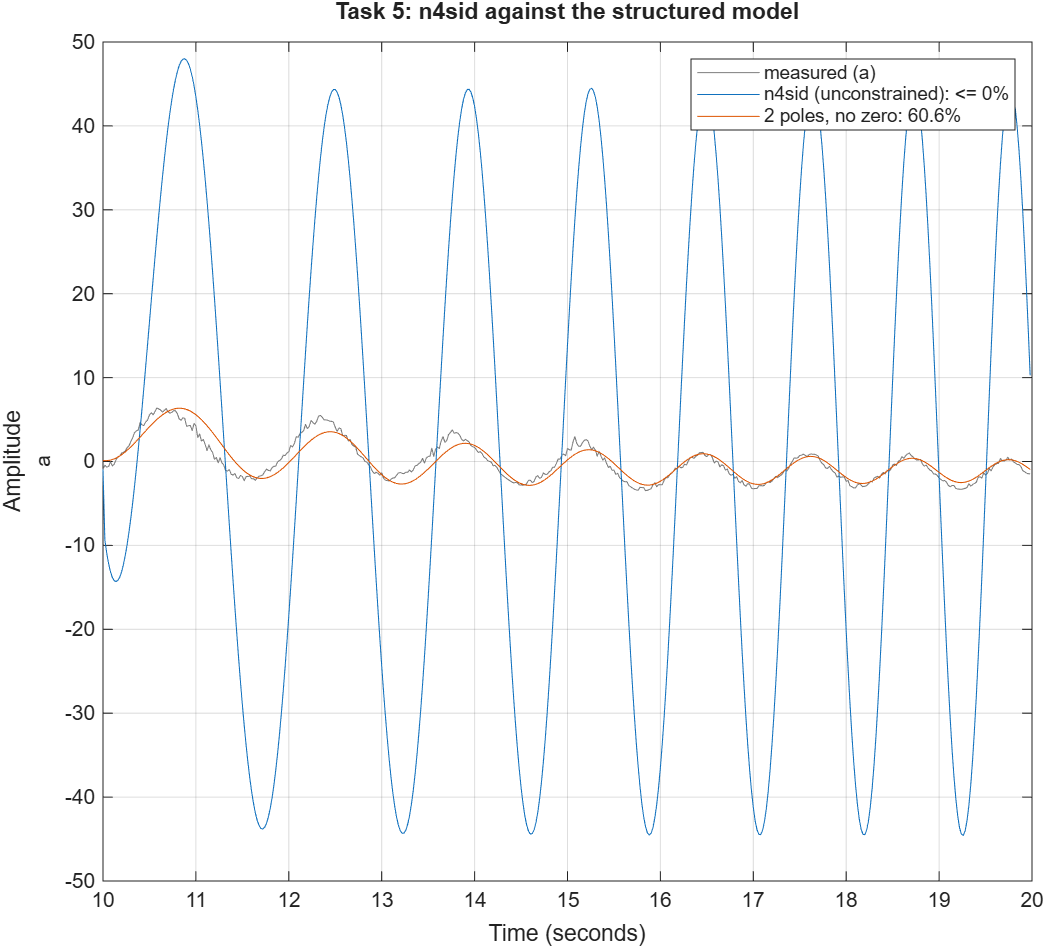
\includegraphics[width=0.92\linewidth]{figures/fig03.png}
\caption{Trial 1: unconstrained n4sid (fit 0 \% or less) against the structured
two pole model (fit 60.6 \%).}\label{fig:3}
\end{figure}

\begin{figure}[H]\centering
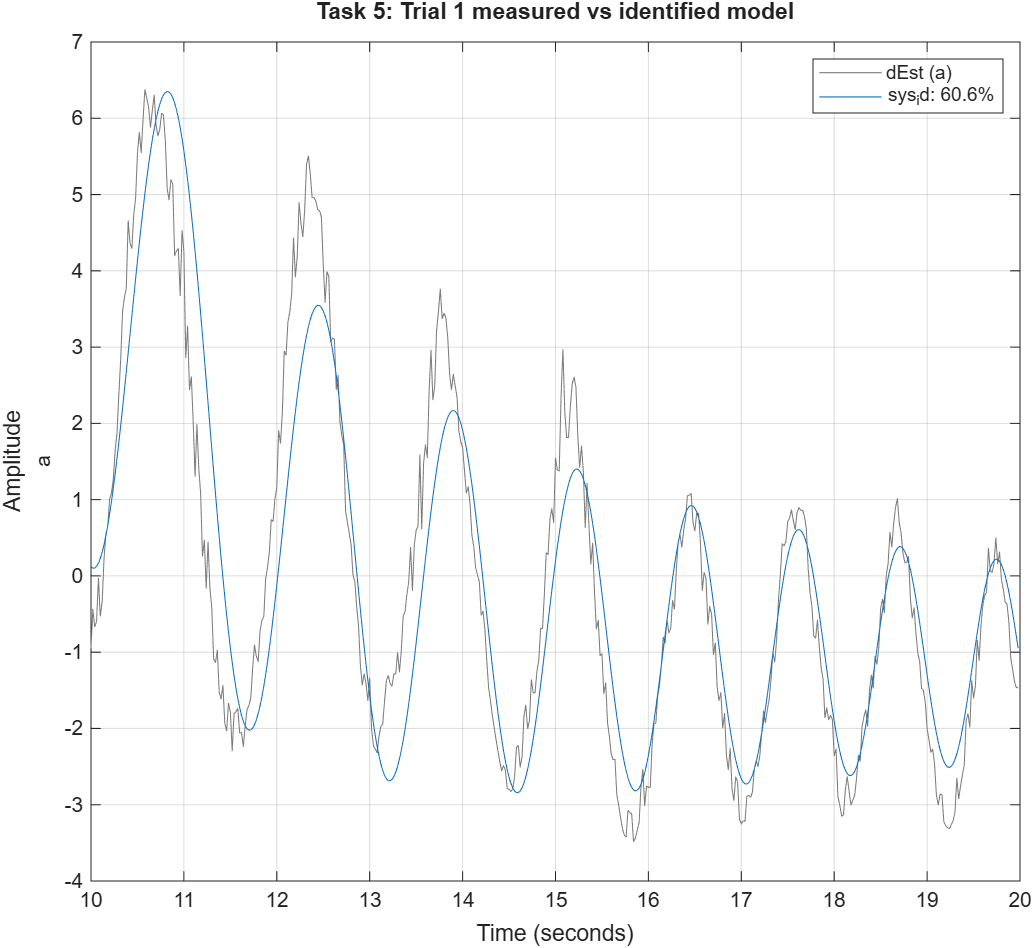
\includegraphics[width=0.92\linewidth]{figures/fig04.png}
\caption{Trial 1 measured position against the identified model.}\label{fig:4}
\end{figure}

\hypertarget{what-the-model-means-physically}{%
\subsection{What the model means
physically}\label{what-the-model-means-physically}}

\begin{itemize}
\tightlist
\item
  Pole at -0.0054 rad/s: practically at the origin. The car integrates
  its velocity into position, exactly as in Part 1.
\item
  Pole at -0.474 rad/s: a slow drag from rolling resistance, time
  constant 1/0.474 = 2.1 s. Part 1 neglected it, which gave a pure
  double integrator. Writing G(s) as 2.591/((s + 0.474)(s + 0.0054))
  shows the model is ``double integrator plus a little damping''.
\item
  Gain 2.591 cm/(deg s²): 76 \% of the Part 1 value 3.424. Friction and
  wheel inertia absorb part of the push from the tilted beam.
\end{itemize}

\hypertarget{validation}{%
\subsection{Validation}\label{validation}}

\textbf{Table 2: Fit of the identified model on every trial}

\begin{longtable}[]{@{}
  >{\raggedright\arraybackslash}p{(\columnwidth - 4\tabcolsep) * \real{0.3333}}
  >{\raggedright\arraybackslash}p{(\columnwidth - 4\tabcolsep) * \real{0.3333}}
  >{\raggedright\arraybackslash}p{(\columnwidth - 4\tabcolsep) * \real{0.3333}}@{}}
\toprule\noalign{}
\begin{minipage}[b]{\linewidth}\raggedright
Data set
\end{minipage} & \begin{minipage}[b]{\linewidth}\raggedright
Fit
\end{minipage} & \begin{minipage}[b]{\linewidth}\raggedright
Reason
\end{minipage} \\
\midrule\noalign{}
\endhead
\bottomrule\noalign{}
\endlastfoot
Trial 1 (estimation) & 60.6 \% & clean, large motion \\
Trial 2 & 14.1 \% & car pressed against the sensor end for 3.3 s: the
output was clipped \\
Trial 3 & 46.6 \% & small motion, but the model follows the trend \\
Trial 4 & 16.1 \% & motion only 0.5 to 2 cm, friction and sensor noise
dominate \\
\end{longtable}

\begin{figure}[H]\centering
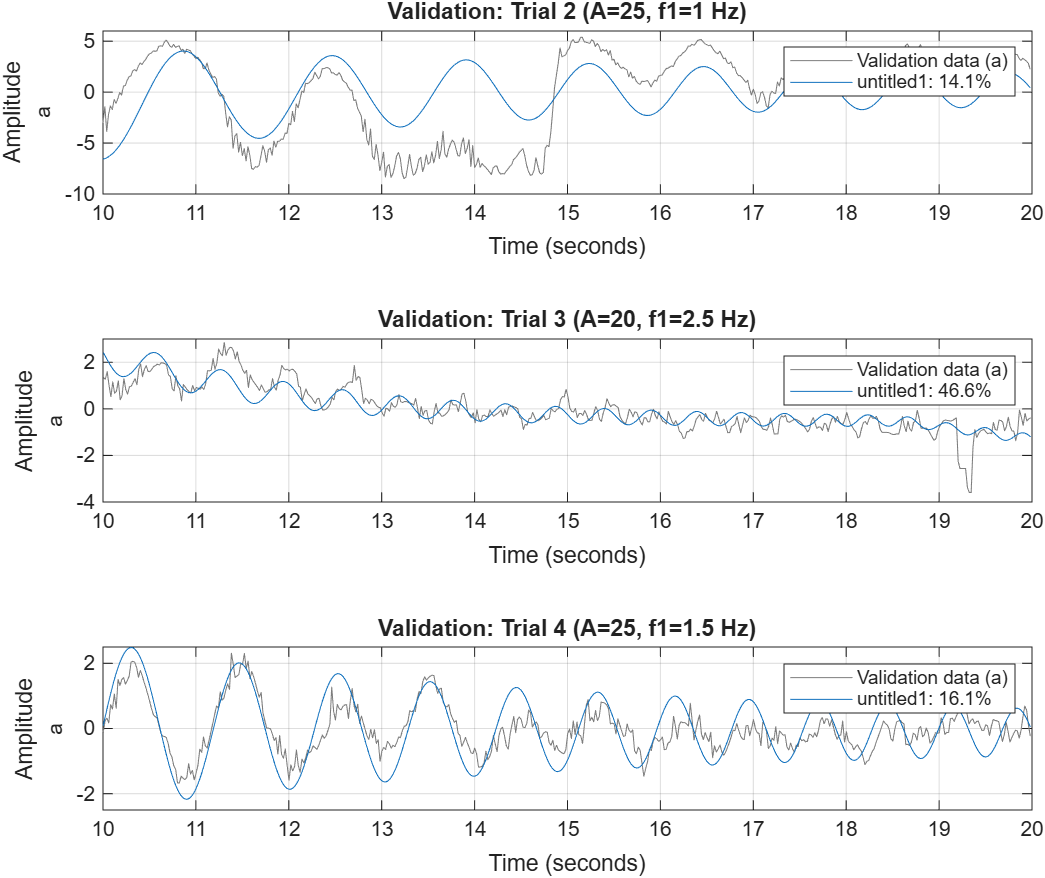
\includegraphics[width=0.92\linewidth]{figures/fig05.png}
\caption{Validation of the identified model on trials 2, 3 and 4.}\label{fig:5}
\end{figure}

The model is reliable for motions of a few centimetres around 1 to 8
rad/s. For very small motions the stick slip of the wheels makes the car
respond less than any linear model predicts, which is why trial 4 fits
poorly.

\hypertarget{bode-plot-analysis}{%
\subsection{Bode plot analysis}\label{bode-plot-analysis}}

Besides the model, we measured the gain and phase directly from each
trial. In windows of 1.5 chirp cycles we fitted y = a sin φ + b cos φ +
c + d t to the position and the same form to the servo angle (φ is the
chirp phase). The ratio of the two complex amplitudes gives
\textbar G(jω)\textbar{} and ∠G(jω) at the frequency of that window.

\begin{figure}[H]\centering
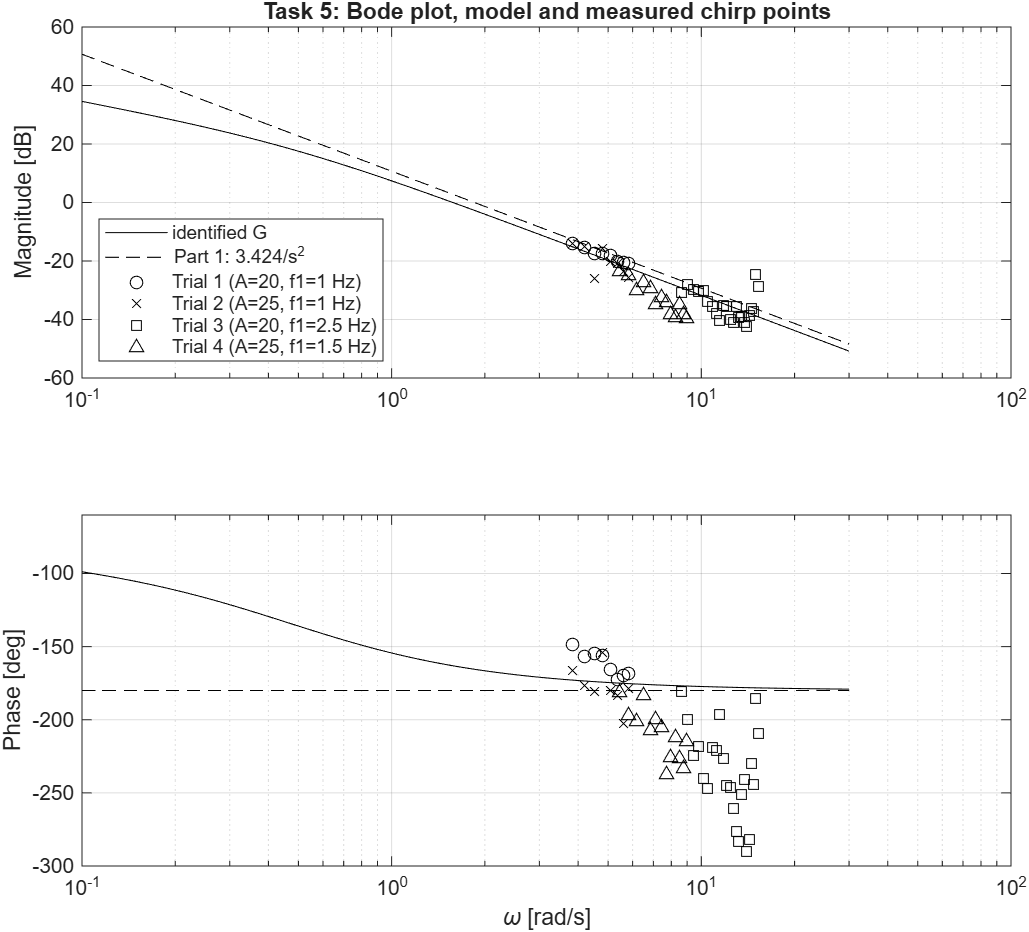
\includegraphics[width=0.92\linewidth]{figures/fig06.png}
\caption{Bode plot of the identified model (solid), the Part 1 model (dashed) and
the gain and phase measured from each trial (markers).}\label{fig:6}
\end{figure}

\begin{itemize}
\tightlist
\item
  Magnitude: above about 1 rad/s the model falls at -40 dB per decade,
  the slope of a double integrator, and lies just below the Part 1 line.
  The trial 1 points sit on the model between 3.8 and 6 rad/s.
\item
  Low frequency: below about 0.47 rad/s the slope eases to -20 dB per
  decade because of the drag pole. The chirp had no data there, so this
  part is set by the fit, not by measurement.
\item
  Phase: the model runs from about -100 deg to -180 deg. The phase
  measured in trials 3 and 4 keeps dropping to between -200 and -280 deg
  at 6 to 14 rad/s, while the gain stays near the model. A falling phase
  with unchanged gain is the signature of a time delay, which adds a
  phase of -ωTd. About 60 deg (1.05 rad) extra at 10 rad/s means Td ≈
  0.1 s. This matches the 70 ms servo and sensor delay from Part 1 plus
  half of the 40 ms control period, so every design below is also
  checked with an extra 90 ms delay.
\end{itemize}

\hypertarget{task-6-root-locus-nyquist-and-bode-analysis}{%
\section{Task 6: Root locus, Nyquist and Bode
analysis}\label{task-6-root-locus-nyquist-and-bode-analysis}}

\emph{What the task asks: plot the root locus and Nyquist diagram of the
open loop transfer function and discuss stability and robustness; plot
the Bode diagram and interpret the gain and phase margins; check the
design criteria (overshoot under 5 \%, settling under 5 s) on the
uncompensated loop.}

The loop studied is a proportional gain K in unity feedback around G(s):
the servo angle is K times the position error. Each plot was made with
and without the 90 ms delay (a third order Pade approximation in
MATLAB).

\hypertarget{root-locus}{%
\subsection{Root locus}\label{root-locus}}

\begin{figure}[H]\centering
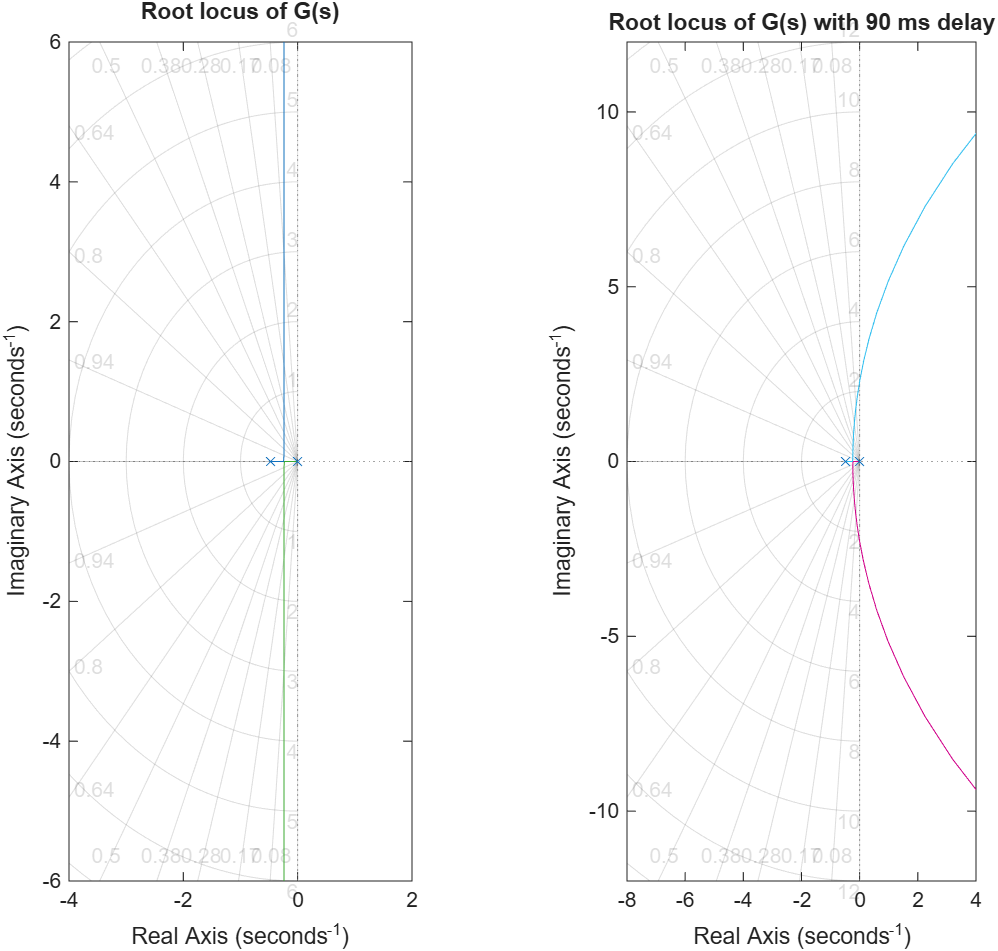
\includegraphics[width=0.92\linewidth]{figures/fig07.png}
\caption{Root locus of G(s), without (left) and with (right) the 90 ms delay.}\label{fig:7}
\end{figure}

How the locus is built (standard rules):

\begin{itemize}
\tightlist
\item
  Branches start at the open loop poles (-0.0054 and -0.4735) and, with
  no finite zeros, go to infinity.
\item
  The real axis between the two poles is part of the locus (odd number
  of poles to the right).
\item
  Two branches go to infinity along asymptotes at ±90 deg, centred at
  (sum of poles)/2 = -0.24.
\item
  The branches meet on the real axis at the breakaway point s = -0.24
  and then run straight up and down the line Re(s) = -0.24.
\end{itemize}

What it tells us:

\begin{itemize}
\tightlist
\item
  At K = 1 the closed loop poles are s = -0.2395 ± 1.5927j, so ωn = 1.61
  rad/s and ζ = 0.149: very lightly damped.
\item
  Without delay the loop is stable for every K \textgreater{} 0, but
  raising K only moves the poles further up the vertical line. The real
  part stays at -0.24, so the 5 \% settling time can never be shorter
  than 3/0.24 = 12.5 s, and the damping keeps falling as K rises. A gain
  alone cannot meet the specifications.
\item
  With the delay the branches bend into the right half plane. They cross
  the imaginary axis at 2.29 rad/s when K = 2.07, so doubling the gain
  would make the real loop unstable.
\end{itemize}

\hypertarget{nyquist-plot}{%
\subsection{Nyquist plot}\label{nyquist-plot}}

\begin{figure}[H]\centering
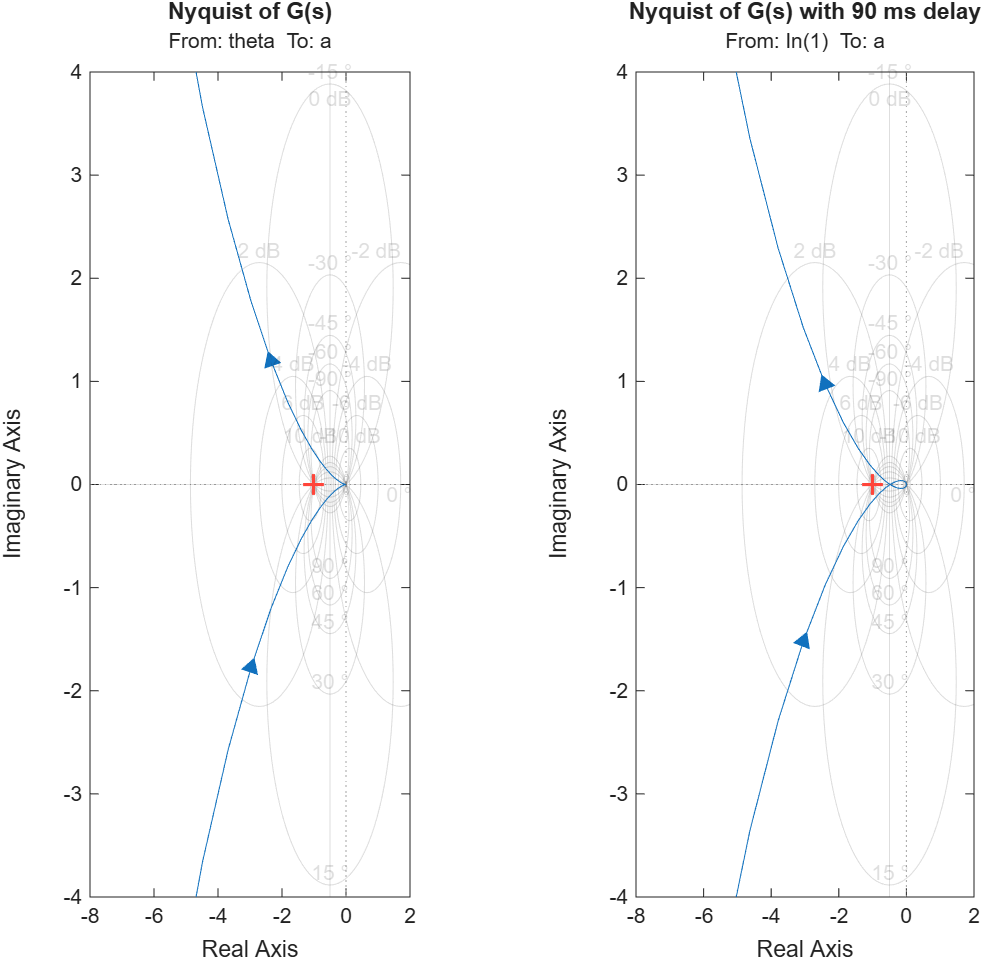
\includegraphics[width=0.92\linewidth]{figures/fig08.png}
\caption{Nyquist plot of G(s), without and with the 90 ms delay.}\label{fig:8}
\end{figure}

The Nyquist criterion is Z = P - N, where P is the number of open loop
poles in the right half plane, N the number of counter clockwise
encirclements of -1, and Z the number of unstable closed loop poles.

\begin{itemize}
\tightlist
\item
  G(s) has no right half plane poles (P = 0) and the curve does not
  encircle -1 (N = 0), so Z = 0 and the unity feedback loop is stable,
  in agreement with the root locus.
\item
  Robustness is poor: the curve passes close to -1. The smallest
  distance is 0.28, which means a peak sensitivity Ms = 1/0.28 = 3.5.
  With the delay it falls to 0.15 (Ms = 6.8). A well designed loop has
  Ms below about 2.
\item
  With the delay a small loop appears near the origin and the curve
  crosses the negative real axis at -0.48. Multiplying the gain by
  1/0.48 = 2.07 would put that crossing on -1, the same limit the root
  locus gave.
\end{itemize}

\hypertarget{bode-plot-gain-and-phase-margin}{%
\subsection{Bode plot, gain and phase
margin}\label{bode-plot-gain-and-phase-margin}}

\begin{figure}[H]\centering
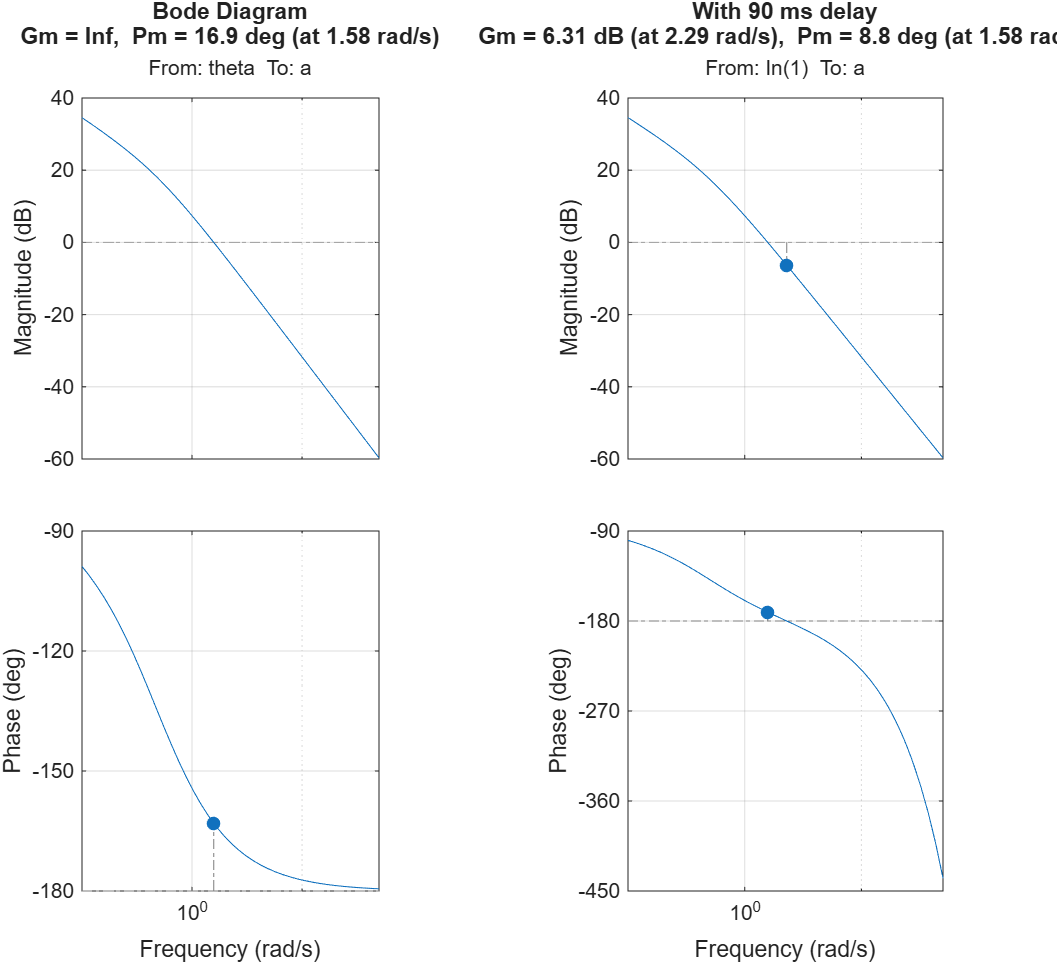
\includegraphics[width=0.92\linewidth]{figures/fig09.png}
\caption{Open loop Bode plots with the margins marked by MATLAB.}\label{fig:9}
\end{figure}

Phase margin (PM) is how far the phase is above -180 deg at the
frequency where the gain is 0 dB. Gain margin (GM) is how much the gain
can be multiplied before the loop goes unstable, read where the phase is
-180 deg. Delay margin is PM (in radians) divided by the crossover
frequency.

\textbf{Table 3: Margins without a compensator}

\begin{longtable}[]{@{}
  >{\raggedright\arraybackslash}p{(\columnwidth - 6\tabcolsep) * \real{0.2500}}
  >{\raggedright\arraybackslash}p{(\columnwidth - 6\tabcolsep) * \real{0.2500}}
  >{\raggedright\arraybackslash}p{(\columnwidth - 6\tabcolsep) * \real{0.2500}}
  >{\raggedright\arraybackslash}p{(\columnwidth - 6\tabcolsep) * \real{0.2500}}@{}}
\toprule\noalign{}
\begin{minipage}[b]{\linewidth}\raggedright
Loop
\end{minipage} & \begin{minipage}[b]{\linewidth}\raggedright
Phase margin
\end{minipage} & \begin{minipage}[b]{\linewidth}\raggedright
Gain margin
\end{minipage} & \begin{minipage}[b]{\linewidth}\raggedright
Delay margin
\end{minipage} \\
\midrule\noalign{}
\endhead
\bottomrule\noalign{}
\endlastfoot
G(s) & 16.9 deg at 1.58 rad/s & infinite (phase never reaches -180 deg)
& 0.188 s \\
G(s) with 90 ms delay & 8.8 deg at 1.58 rad/s & 2.07 (6.31 dB) at 2.29
rad/s & 0.098 s \\
Part 1 model 3.424/s² & 0 deg at 1.85 rad/s & not defined & 0 s \\
\end{longtable}

How the three views agree:

\begin{itemize}
\tightlist
\item
  The gain margin of 2.07 at 2.29 rad/s (with delay) is the same gain
  and frequency where the delayed root locus crosses the imaginary axis
  and where the Nyquist curve would pass through -1.
\item
  A phase margin of 16.9 deg corresponds to ζ ≈ PM/100 ≈ 0.17, close to
  the ζ = 0.149 of the root locus poles and to the Nyquist curve passing
  close to -1.
\item
  The delay margin of 0.188 s says the loop tolerates only 0.19 s of
  extra delay. The hardware already has about 0.09 s, which is why the
  margins halve with the delay.
\end{itemize}

\hypertarget{design-criteria}{%
\subsection{Design criteria}\label{design-criteria}}

The specifications are turned into frequency domain targets with the
standard second order relations:

\texttt{ζ\ =\ -ln(OS)\ /\ √(π²\ +\ ln²(OS))\ =\ 0.690\ \ \ for\ OS\ =\ 5\ \%}

\texttt{PM\ =\ atan(\ 2ζ\ /\ √(\ √(1\ +\ 4ζ⁴)\ -\ 2ζ²\ )\ )\ =\ 64.6\ deg,\ \ \ \ \ \ \ \ Ts(5\ \%)\ ≈\ 3/(ζ\ ωn)\ \textless{}\ 5\ s\ \ →\ \ ζ\ ωn\ \textgreater{}\ 0.6\ rad/s}

\begin{figure}[H]\centering
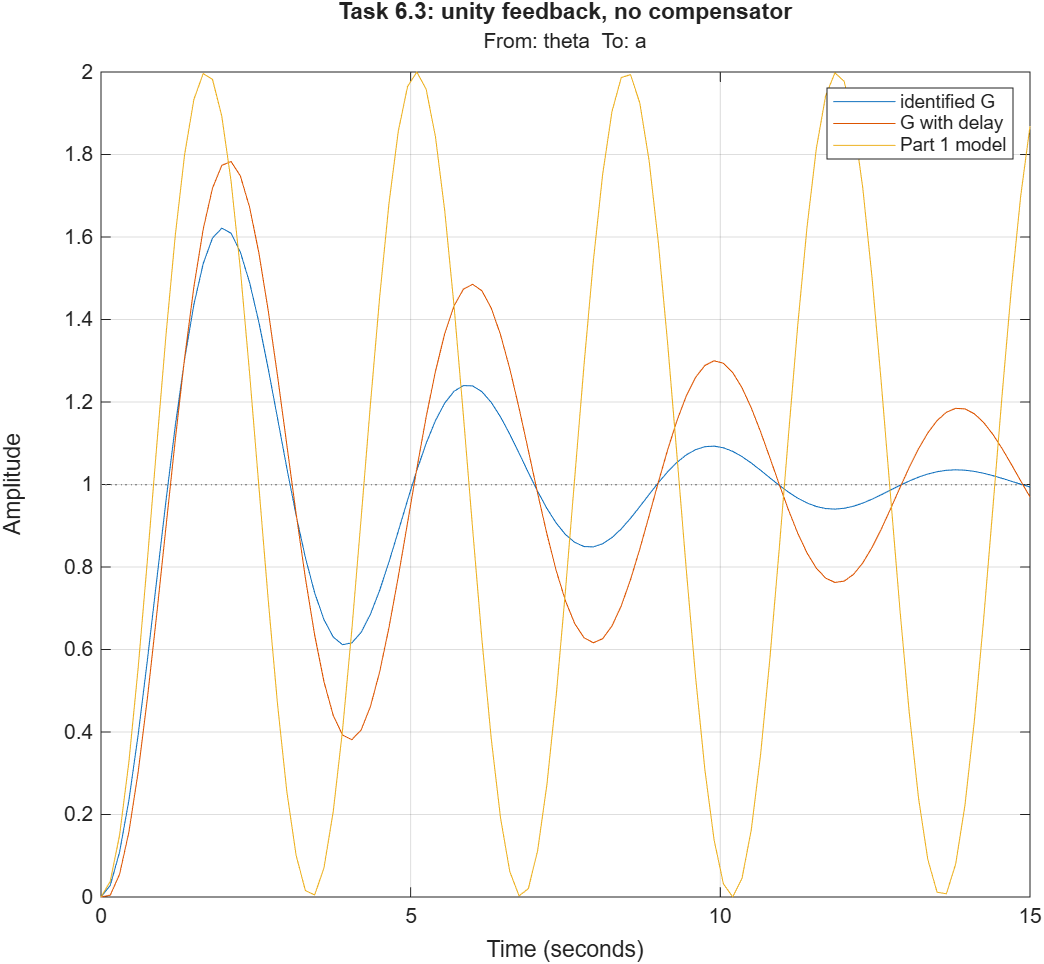
\includegraphics[width=0.92\linewidth]{figures/fig10.png}
\caption{Unity feedback step responses without a compensator.}\label{fig:10}
\end{figure}

\textbf{Table 4: Uncompensated performance}

\begin{longtable}[]{@{}llll@{}}
\toprule\noalign{}
Case & Overshoot & Settling time (5 \%) & Meets specs? \\
\midrule\noalign{}
\endhead
\bottomrule\noalign{}
\endlastfoot
Identified G(s) & 62.2 \% & 12.18 s & No \\
G(s) with 90 ms delay & 78.7 \% & 24.0 s & No \\
Part 1 model & 100 \%, never settles & none & No \\
\end{longtable}

The loop has 16.9 deg of phase margin (8.8 deg with delay) against the
64.6 deg needed, and ζωn = 0.24 rad/s against the 0.6 rad/s needed. Both
specifications fail and the root locus shows a gain cannot fix them.
About 50 deg of extra phase is needed near the crossover frequency.

\hypertarget{task-7-lead-or-lag-compensator}{%
\section{Task 7: Lead or lag
compensator}\label{task-7-lead-or-lag-compensator}}

\emph{What the task asks: from the frequency domain results, identify
and design the required lead or lag compensator for the desired
transient and steady state performance, and verify the improvement with
Bode plots and step responses.}

\hypertarget{lead-or-lag}{%
\subsection{Lead or lag?}\label{lead-or-lag}}

\begin{itemize}
\tightlist
\item
  A lead compensator, C(s) = Kc (Ts + 1)/(αTs + 1) with α \textless{} 1,
  adds positive phase around its centre frequency. Phase margin is what
  Task 6 showed is missing, so lead is the direct fix for overshoot and
  damping.
\item
  A lag compensator, with α \textgreater{} 1, raises the low frequency
  gain to cut steady state error, but it adds negative phase. On its own
  it can only lower the crossover frequency to where the plant phase is
  better, which makes the loop slow.
\item
  Our model already has a pole almost at the origin, so in the linear
  model the steady state error is already near zero. The real reason a
  lag stage can help is friction: it raises the gain at low frequency so
  that a small remaining error still produces enough servo angle to move
  the car. We therefore designed all three options and compared them.
\end{itemize}

\hypertarget{lead-design-step-by-step}{%
\subsection{Lead design, step by step}\label{lead-design-step-by-step}}

\begin{enumerate}
\def\labelenumi{\arabic{enumi}.}
\tightlist
\item
  Choose the crossover ωc = 4 rad/s. It is well above the ζωn
  \textgreater{} 0.6 limit, high enough for the gain to fight friction
  on the hardware, and low enough that the 90 ms delay only costs ωc Td
  = 21 deg.
\item
  Choose α = 0.1, which gives up to φmax = asin((1 - α)/(1 + α)) = 54.9
  deg of phase lead.
\item
  Put the peak lead at ωc: T = 1/(ωc √α) = 0.791 s, so αT = 0.0791 s.
  The zero is at -1.265 rad/s and the pole at -12.65 rad/s.
\item
  Choose Kc so that the loop gain is 1 at ωc: \textbar Kc C0(jωc)
  G(jωc)\textbar{} = 1 gives Kc = 1.966 deg/cm.
\item
  Add a prefilter F(s) = 1/(Ts + 1) on the target. The lead zero appears
  in the closed loop and causes 13 \% overshoot on its own. The
  prefilter cancels it for target changes only; stability and
  disturbance rejection are unchanged. This is the same idea as the
  derivative on measurement (c = 0) of Part 1.
\end{enumerate}

\texttt{C\_lead(s)\ =\ 1.966\ (0.791\ s\ +\ 1)\ /\ (0.0791\ s\ +\ 1),\ \ \ \ \ \ \ \ F(s)\ =\ 1\ /\ (0.791\ s\ +\ 1)}

\begin{figure}[H]\centering
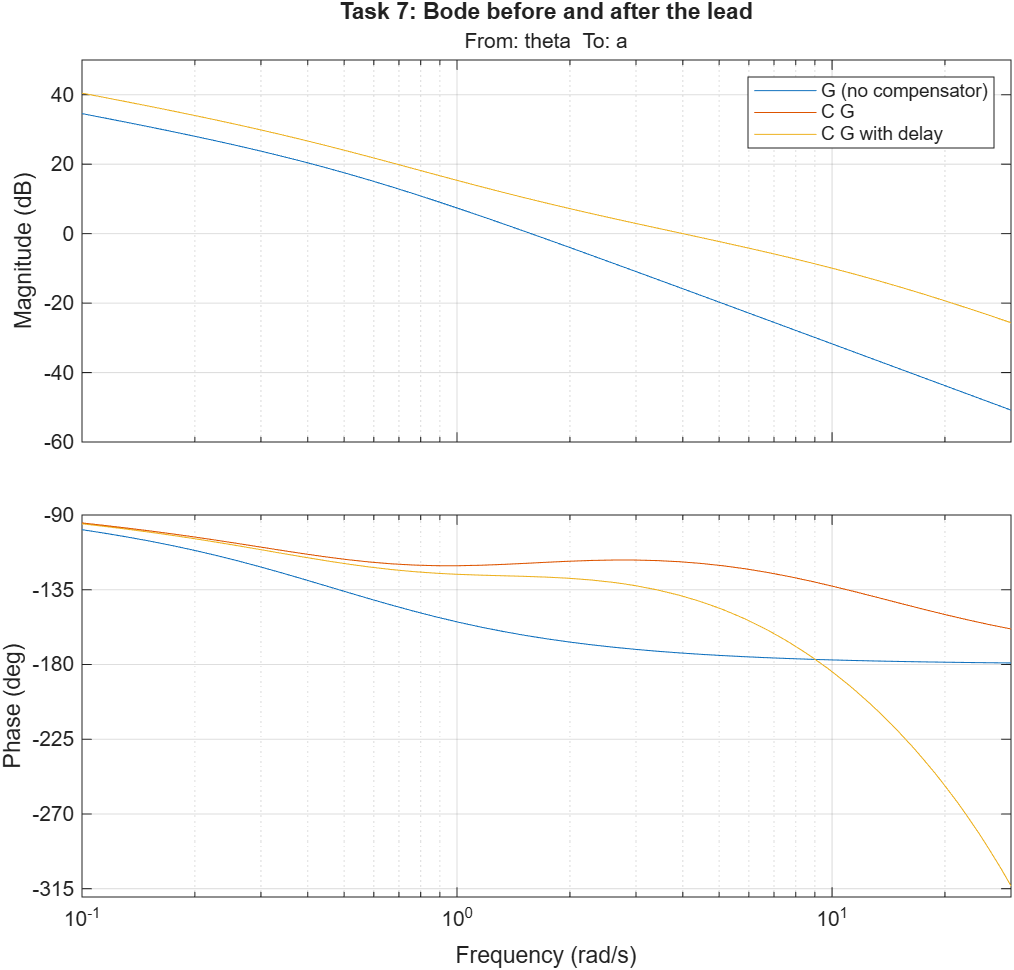
\includegraphics[width=0.92\linewidth]{figures/fig11.png}
\caption{Open loop Bode plot before and after the lead compensator.}\label{fig:11}
\end{figure}

\begin{figure}[H]\centering
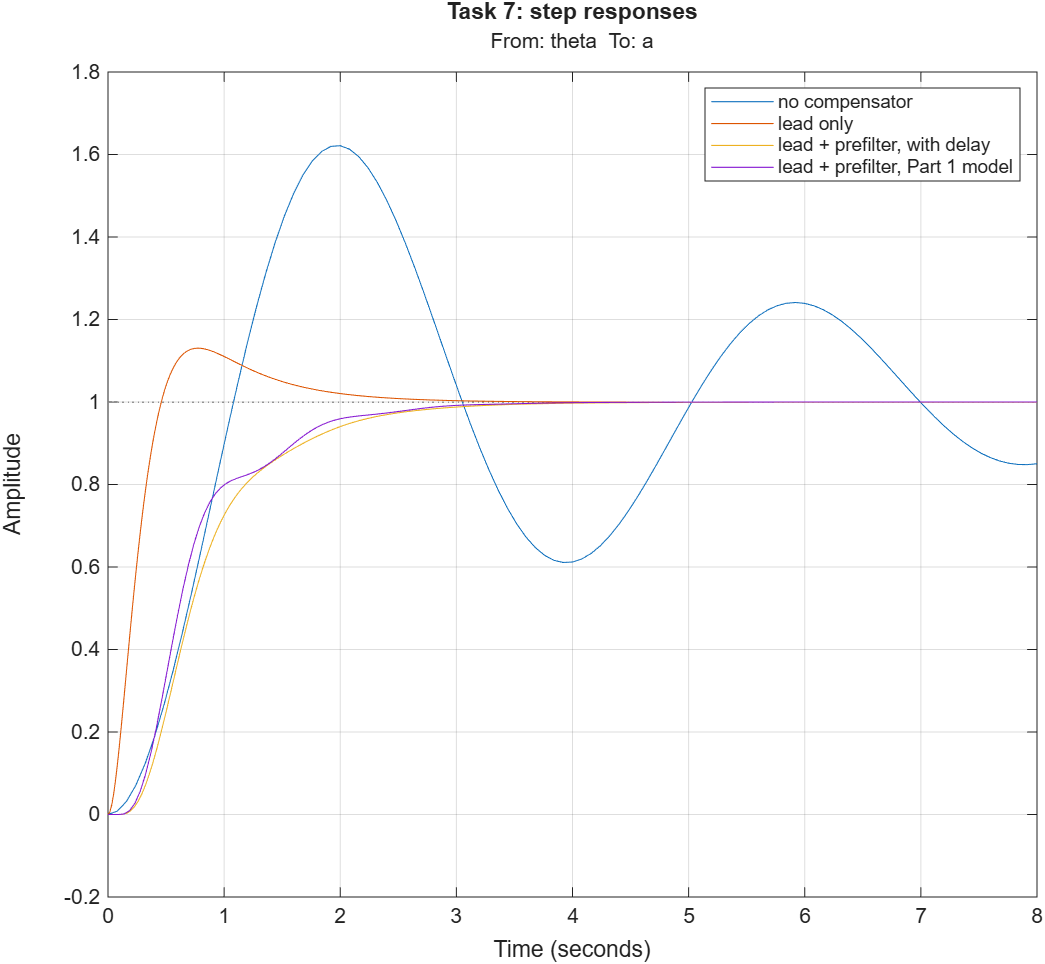
\includegraphics[width=0.92\linewidth]{figures/fig12.png}
\caption{Step responses before and after the lead compensator.}\label{fig:12}
\end{figure}

\begin{figure}[H]\centering
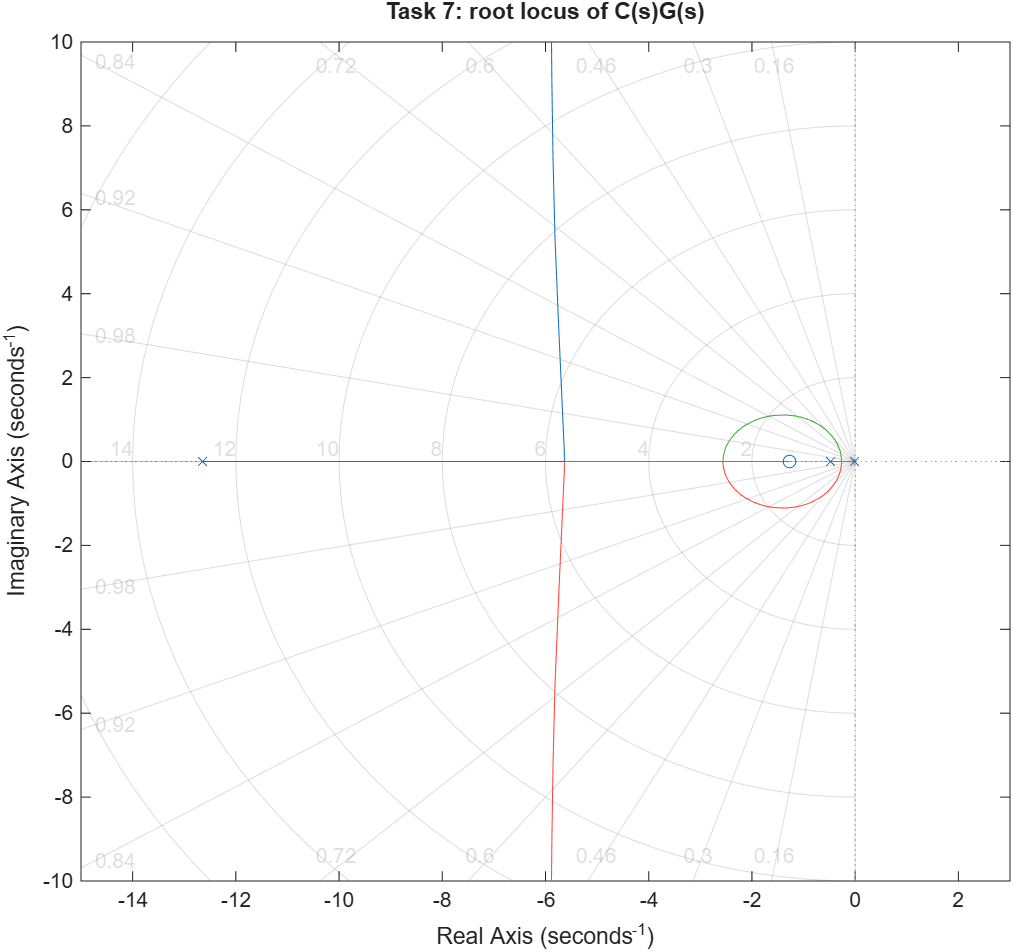
\includegraphics[width=0.92\linewidth]{figures/fig13.png}
\caption{Root locus with the lead. The zero at -1.265 pulls the branches far into
the left half plane.}\label{fig:13}
\end{figure}

With the lead the closed loop poles move from -0.24 ± 1.59j to -5.70 ±
2.19j and -1.73. The dominant real part is about 24 times further left,
so settling drops from 12.2 s to about 2 s while the damping rises.

\hypertarget{lag-design}{%
\subsection{Lag design}\label{lag-design}}

For comparison a lag alone was designed to give about 50 deg of phase
margin. The plant phase is -125 deg at 0.343 rad/s, so the crossover was
moved there by lowering the high frequency gain to
1/\textbar G(j0.343)\textbar{} = 0.0774, with the lag zero a decade
below (0.0343 rad/s) and unity gain at DC:

\texttt{C\_lag(s)\ =\ 0.0774\ (s\ +\ 0.0343)\ /\ (s\ +\ 0.00265)}

\hypertarget{lead-lag-design}{%
\subsection{Lead-lag design}\label{lead-lag-design}}

The lead was kept and a lag stage was added well below the crossover
(zero at ωc/20 = 0.2 rad/s, pole at 0.02 rad/s, so the low frequency
gain rises 10 times while the gain near ωc is almost unchanged):

\texttt{C\_LL(s)\ =\ 1.966\ (0.791\ s\ +\ 1)/(0.0791\ s\ +\ 1)\ x\ (s\ +\ 0.2)/(s\ +\ 0.02),\ \ \ with\ the\ same\ prefilter\ F(s)}

\hypertarget{comparison-and-choice}{%
\subsection{Comparison and choice}\label{comparison-and-choice}}

\begin{figure}[H]\centering
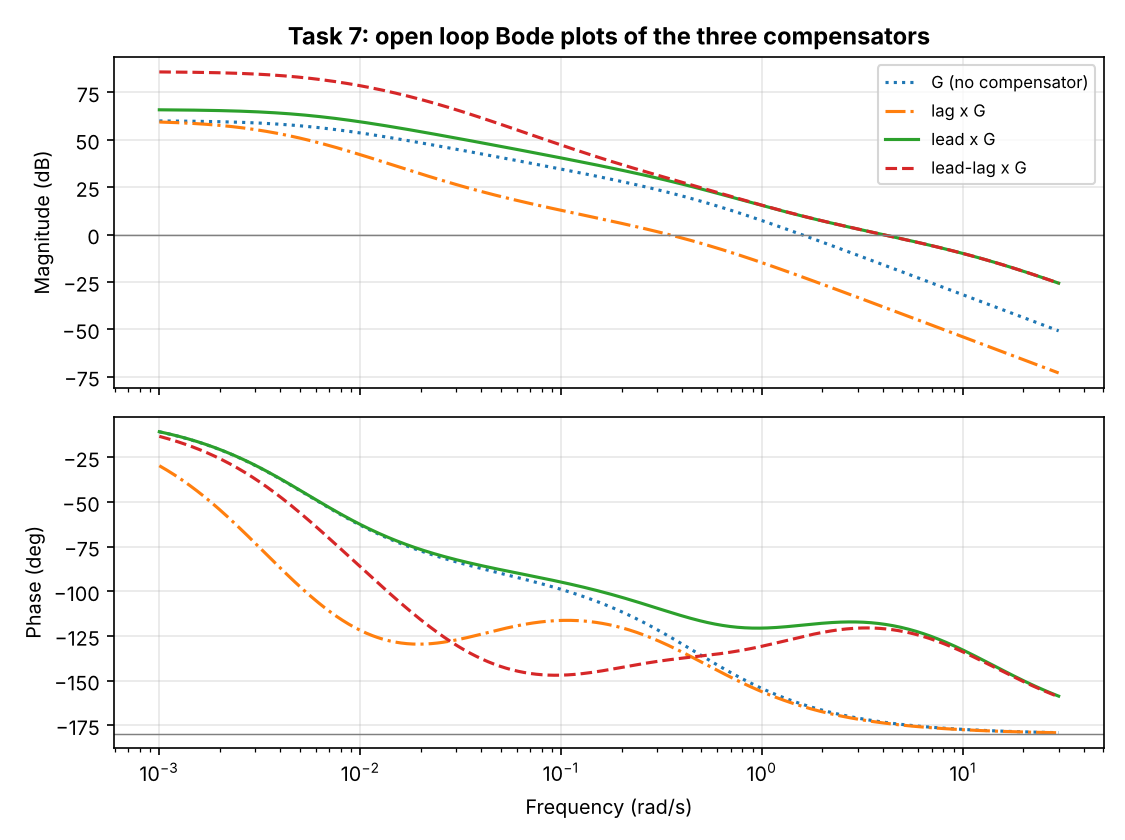
\includegraphics[width=0.92\linewidth]{figures/fig14.png}
\caption{Open loop Bode plots of the plant with each compensator.}\label{fig:14}
\end{figure}

\begin{figure}[H]\centering
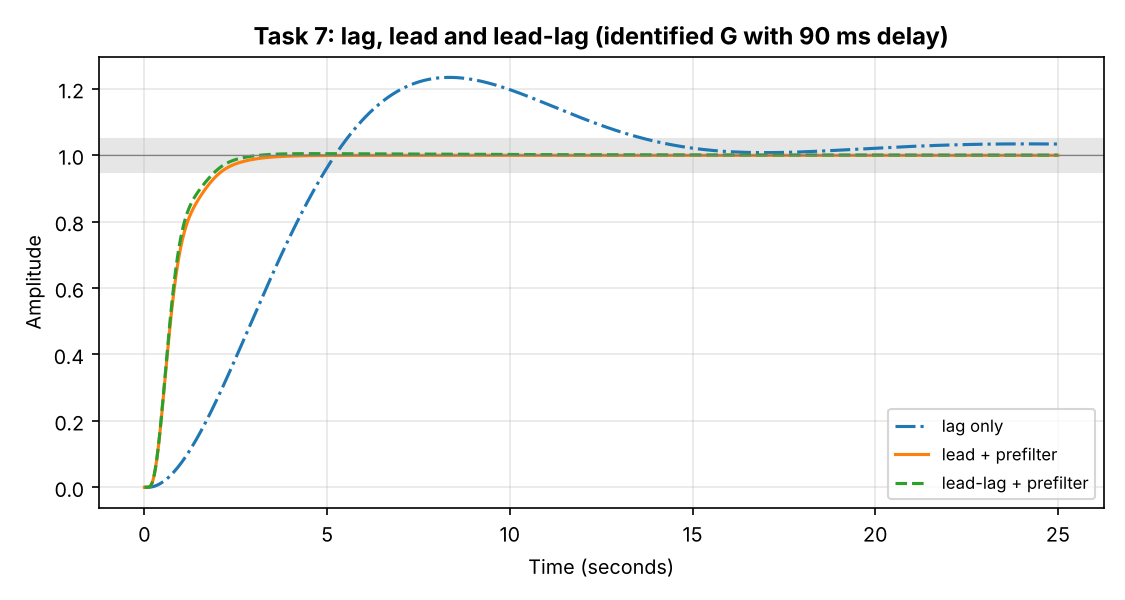
\includegraphics[width=0.92\linewidth]{figures/fig15.png}
\caption{Closed loop step responses with each compensator (identified model with
90 ms delay).}\label{fig:15}
\end{figure}

\textbf{Table 5: Simulated results on the identified model (time results
include the 90 ms delay)}

\begin{longtable}[]{@{}
  >{\raggedright\arraybackslash}p{(\columnwidth - 10\tabcolsep) * \real{0.1667}}
  >{\raggedright\arraybackslash}p{(\columnwidth - 10\tabcolsep) * \real{0.1667}}
  >{\raggedright\arraybackslash}p{(\columnwidth - 10\tabcolsep) * \real{0.1667}}
  >{\raggedright\arraybackslash}p{(\columnwidth - 10\tabcolsep) * \real{0.1667}}
  >{\raggedright\arraybackslash}p{(\columnwidth - 10\tabcolsep) * \real{0.1667}}
  >{\raggedright\arraybackslash}p{(\columnwidth - 10\tabcolsep) * \real{0.1667}}@{}}
\toprule\noalign{}
\begin{minipage}[b]{\linewidth}\raggedright
Compensator
\end{minipage} & \begin{minipage}[b]{\linewidth}\raggedright
Phase margin (no delay)
\end{minipage} & \begin{minipage}[b]{\linewidth}\raggedright
Phase margin / gain margin with 90 ms delay
\end{minipage} & \begin{minipage}[b]{\linewidth}\raggedright
Overshoot
\end{minipage} & \begin{minipage}[b]{\linewidth}\raggedright
Settling (5 \%)
\end{minipage} & \begin{minipage}[b]{\linewidth}\raggedright
Specs?
\end{minipage} \\
\midrule\noalign{}
\endhead
\bottomrule\noalign{}
\endlastfoot
None & 16.9 deg & 8.8 deg / 2.07 & 78.7 \% & 24.0 s & No \\
Lag only & 49.6 deg at 0.34 rad/s & 47.9 deg / 25.0 & 23.5 \% & 13.7 s &
No \\
Lead + prefilter & 61.7 deg at 4.0 rad/s & 41.1 deg / 2.89 & 0 \% & 2.10
s & Yes \\
Lead-lag + prefilter & 59.2 deg at 4.0 rad/s & 38.5 deg / 2.83 & 0.4 \%
& 1.94 s & Yes \\
\end{longtable}

\begin{itemize}
\tightlist
\item
  The lag alone cannot meet the specifications: it buys phase margin
  only by making the loop about 12 times slower, and its gain of 0.08
  deg/cm is far too small to overcome friction on the hardware.
\item
  The lead meets both specifications with margin to spare. It is the
  compensator required by the frequency domain analysis.
\item
  The lead-lag meets them as well, costs only 2.5 deg of phase margin,
  and multiplies the low frequency gain by 10. It was taken to the
  hardware alongside the lead to deal with friction.
\end{itemize}

\hypertarget{why-the-lead-looks-better-than-the-lead-lag-here}{%
\subsection{Why the lead looks better than the lead-lag
here}\label{why-the-lead-looks-better-than-the-lead-lag-here}}

In Table 5 the lead gives 0 \% overshoot with 61.7 deg of phase margin,
while the lead-lag gives 0.4 \% overshoot with 59.2 deg. So on the model
the plain lead is the cleaner design. There are three reasons.

\begin{enumerate}
\def\labelenumi{\arabic{enumi}.}
\tightlist
\item
  The lag stage costs a little phase. Its zero is at 0.2 rad/s and its
  pole at 0.02 rad/s. At the crossover ωc = 4 rad/s the phase it adds is
  tan⁻¹(4/0.2) - tan⁻¹(4/0.02) = 87.1 - 89.7 = -2.5 deg. That is exactly
  the drop from 61.7 to 59.2 deg, and slightly less phase margin means
  slightly less damping, hence the 0.4 \% overshoot.
\item
  The lag solves a problem the model does not have. Its job is to raise
  the low frequency gain 10 times so that the steady state error goes
  away. The identified G(s) already has a pole almost at the origin
  (-0.0054 rad/s), so it behaves like an integrator and the lead alone
  already gives almost zero steady state error. On the model the lag
  brings only its small phase cost.
\item
  The model has no friction. The linear G(s) leaves out the wheel dead
  band, so in simulation nothing stops the car short of the target.
\end{enumerate}

On the hardware the third point changes everything. Friction held the
car 1.7 to 4.8 cm short with the lead alone, and the extra low frequency
gain of the lag stage kept building the servo angle until the car moved,
bringing the error down to 0.09 to 0.43 cm (Section 5.3). So the lead is
the best design on the ideal model, and the lead-lag is the best
controller for the real setup.

\hypertarget{task-8-hardware-implementation}{%
\section{Task 8: Hardware
implementation}\label{task-8-hardware-implementation}}

\emph{What the task asks: implement and tune the designed controllers on
the hardware, and demonstrate stable control and the response to small
perturbations.}

\hypertarget{from-s-domain-to-arduino-code}{%
\subsection{From s-domain to Arduino
code}\label{from-s-domain-to-arduino-code}}

The Arduino runs a fixed 40 ms loop, so each first order block was
turned into a difference equation with the Tustin (bilinear) rule s =
(2/Ts)(z - 1)/(z + 1), Ts = 0.04 s. For a block Kc(Ts + 1)/(αTs + 1)
this gives y{[}k{]} = b0 x{[}k{]} + b1 x{[}k-1{]} + a1 y{[}k-1{]} with

\texttt{b0\ =\ Kc\ (2T\ +\ Ts)/(2αT\ +\ Ts),\ \ \ b1\ =\ Kc\ (Ts\ -\ 2T)/(2αT\ +\ Ts),\ \ \ a1\ =\ (2αT\ -\ Ts)/(2αT\ +\ Ts)}

\textbf{Table 6: Discrete coefficients used in the sketch}

\begin{longtable}[]{@{}
  >{\raggedright\arraybackslash}p{(\columnwidth - 6\tabcolsep) * \real{0.2500}}
  >{\raggedright\arraybackslash}p{(\columnwidth - 6\tabcolsep) * \real{0.2500}}
  >{\raggedright\arraybackslash}p{(\columnwidth - 6\tabcolsep) * \real{0.2500}}
  >{\raggedright\arraybackslash}p{(\columnwidth - 6\tabcolsep) * \real{0.2500}}@{}}
\toprule\noalign{}
\begin{minipage}[b]{\linewidth}\raggedright
Block
\end{minipage} & \begin{minipage}[b]{\linewidth}\raggedright
b0
\end{minipage} & \begin{minipage}[b]{\linewidth}\raggedright
b1
\end{minipage} & \begin{minipage}[b]{\linewidth}\raggedright
a1
\end{minipage} \\
\midrule\noalign{}
\endhead
\bottomrule\noalign{}
\endlastfoot
Lead 1.966 (0.791 s + 1)/(0.0791 s + 1) & 16.0876 & -15.2938 & 0.5962 \\
Lag stage (s + 0.2)/(s + 0.02) & 1.003599 & -0.995602 & 0.999200 \\
Lag only 0.0774 (s + 0.0343)/(s + 0.00265) & 0.077416 & -0.077310 &
0.999894 \\
Prefilter 1/(0.791 s + 1) & 0.02467 (on r{[}k{]} and r{[}k-1{]}) & &
0.95065 \\
\end{longtable}

These match the c2d(C, 0.04, `tustin') output of MATLAB. The sketch
ES245\_LeadLag\_Target.ino keeps the Part 1 wiring (TRIG 9, ECHO A2,
servo 11, level 90 deg) and does the following every 40 ms:

\begin{enumerate}
\def\labelenumi{\arabic{enumi}.}
\tightlist
\item
  Read the sensor, ignore a missing echo (keep the last value) and
  smooth lightly: pos = 0.7 new + 0.3 old.
\item
  Pass the target through the prefilter, so a new target glides in
  instead of jumping (lead and lead-lag only).
\item
  Compute the error e = rf - pos and run it through the lead, or through
  the lead and then the lag stage. Each stage is limited to ±30 deg so
  its memory cannot wind up beyond the servo range.
\item
  Add a friction kick of ±3 deg when the car is more than 0.5 cm from
  the target (as in Part 1). The servo itself is limited to ±30 deg; the
  log can show up to ±33 deg because it records the command with the
  kick before that limit.
\item
  Write the servo and print time, target, filtered target, position and
  servo angle.
\end{enumerate}

Serial commands: 1, 2 or 3 choose lead, lag or lead-lag; T x sets the
target to x cm (allowed 8 to 36 cm); S starts and X stops. The control
loop is listed in Appendix B.

\hypertarget{test-procedure}{%
\subsection{Test procedure}\label{test-procedure}}

For each controller the car was placed near one end of the track, a
target was set and the run started. Targets of 10 cm (near the sensor),
22.12 cm (the beam centre) and 35 cm (the far end of the track) were
tested. In some runs friction held the car still away from the target;
it was then given a light push by hand to free it. Each push also acts
as a perturbation, so these moments show how the loop recovers. The lag
only mode was not recorded on the hardware; with a gain of 0.08 deg/cm
it cannot overcome the friction band, as predicted in Section 4.5.

\hypertarget{results}{%
\subsection{Results}\label{results}}

\textbf{Table 7: Hardware results (final error = target minus rest
position; positive means the car stopped short)}

\begin{longtable}[]{@{}
  >{\raggedright\arraybackslash}p{(\columnwidth - 12\tabcolsep) * \real{0.1429}}
  >{\raggedright\arraybackslash}p{(\columnwidth - 12\tabcolsep) * \real{0.1429}}
  >{\raggedright\arraybackslash}p{(\columnwidth - 12\tabcolsep) * \real{0.1429}}
  >{\raggedright\arraybackslash}p{(\columnwidth - 12\tabcolsep) * \real{0.1429}}
  >{\raggedright\arraybackslash}p{(\columnwidth - 12\tabcolsep) * \real{0.1429}}
  >{\raggedright\arraybackslash}p{(\columnwidth - 12\tabcolsep) * \real{0.1429}}
  >{\raggedright\arraybackslash}p{(\columnwidth - 12\tabcolsep) * \real{0.1429}}@{}}
\toprule\noalign{}
\begin{minipage}[b]{\linewidth}\raggedright
Run
\end{minipage} & \begin{minipage}[b]{\linewidth}\raggedright
Start (cm)
\end{minipage} & \begin{minipage}[b]{\linewidth}\raggedright
Rise time 10 to 90 \% (s)
\end{minipage} & \begin{minipage}[b]{\linewidth}\raggedright
Overshoot
\end{minipage} & \begin{minipage}[b]{\linewidth}\raggedright
Rest position (cm)
\end{minipage} & \begin{minipage}[b]{\linewidth}\raggedright
Final error (cm)
\end{minipage} & \begin{minipage}[b]{\linewidth}\raggedright
Servo at rest (deg)
\end{minipage} \\
\midrule\noalign{}
\endhead
\bottomrule\noalign{}
\endlastfoot
Simulation (lead, any target) & & 1.3 & 0 \% & = target & 0 & 0 \\
Lead, T = 10 & 31.7 & did not reach 90 \% & 0 & 14.82 & -4.82 & -12.5 \\
Lead, T = 22.12 & 7.6 & 4.4 & 0 & 20.47 & +1.65 & +6.5 \\
Lead, T = 35 & 6.7 & 1.84 & reading spikes & 35.33 after 38 s & -0.33 &
-0.7 \\
Lead-lag, T = 10 & 39.8 & 1.12 & 0.33 cm (1.1 \%) & 10.15 & -0.15 &
-0.6 \\
Lead-lag, T = 22.12 & 35.3 & see text & 2.1 cm after push & 22.55 &
-0.43 & -1.8 \\
Lead-lag, T = 35 & 7.9 & 1.68 & reading spikes & 35.09 after 14 s &
-0.09 & -0.8 \\
\end{longtable}

\begin{figure}[H]\centering
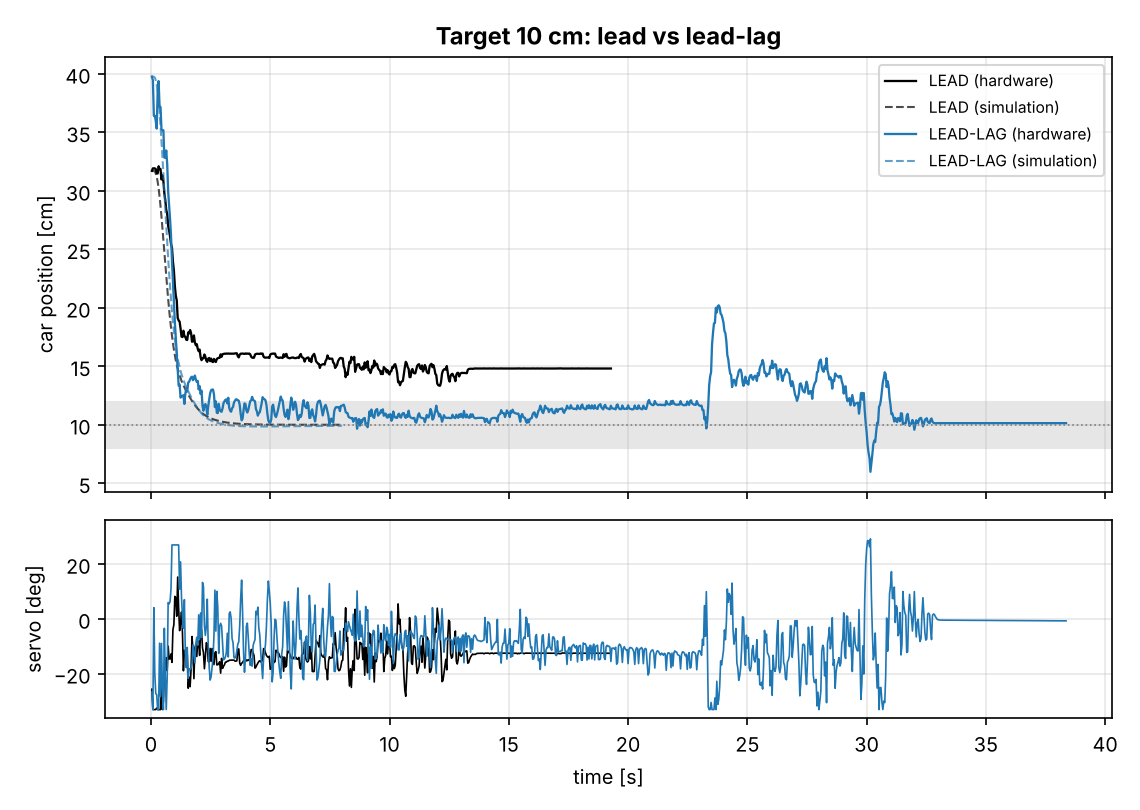
\includegraphics[width=0.92\linewidth]{figures/fig16.png}
\caption{Target 10 cm. Top: car position (solid: hardware, dashed: simulation
from the same start, shaded: ±2 cm band). Bottom: servo command.}\label{fig:16}
\end{figure}

\textbf{Target 10 cm, lead (black).}

The car started at 31.7 cm. The servo went straight to its limit (logged
-33 deg, the servo itself stops at -30 deg; the error was 22 cm), the
car rolled towards the sensor and reached 16 cm in about 1.5 s, close to
the simulated speed. It then stopped at about 15 cm and stayed there,
finishing at 14.82 cm, 4.82 cm short. The servo command at rest was
-12.5 deg, which is exactly what the lead gives for that error: Kc x e -
kick = 1.966 x (-4.82) - 3 = -12.5 deg. The lead has a finite gain at
low frequency, so once the error is small its command stays constant; at
this point of the track that command was not enough to break the static
friction of the wheels, so the car never moved again.

\textbf{Target 10 cm, lead-lag (blue).}

From 39.8 cm the car reached the target region in 1.2 s with only 0.33
cm (1.1 \%) of overshoot, very close to the simulated curve. It then
hunted gently between 10 and 12 cm: every time it stopped, the lag stage
slowly increased the command (its pole at 0.02 rad/s has a 50 s time
constant) until the car broke free and moved a little. Friction kept
holding it between 11 and 12 cm, so at 23.3 s it was pushed by hand to
free it. The push carried it away from the sensor to 20.2 cm (it moved
against a -12 deg command, confirming an external push); the servo went
to its limit and pulled it back to about 13 cm within 1 s, where
friction held it again. A second push at 29.9 s moved it towards the
sensor to 6 cm (again against the command); the controller brought it
back and it settled within ±1 cm of the target 1.1 s after the push, at
10.15 cm, an error of only 0.15 cm. The servo then crept slowly from
-0.4 to -0.7 deg: that is the lag stage integrating the last 0.15 cm of
error.

\begin{figure}[H]\centering
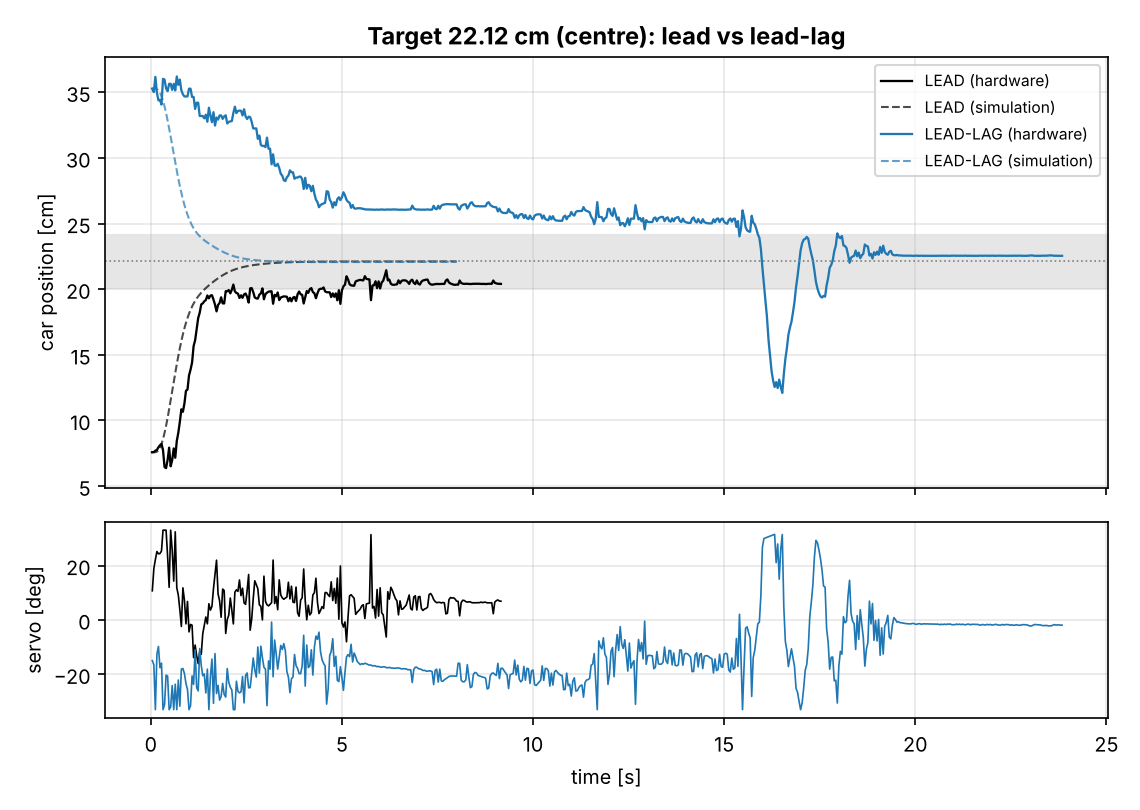
\includegraphics[width=0.92\linewidth]{figures/fig17.png}
\caption{Target 22.12 cm (the beam centre).}\label{fig:17}
\end{figure}

\textbf{Target 22.12 cm, lead (black).}

Starting at 7.6 cm, the car stayed still for 0.7 s while the command
rose to the servo limit (static friction must be overcome first), then
rolled to 19 to 20 cm in about 1.4 s and stopped short of the target. It
rested at 20.47 cm with +6.5 deg of command (1.966 x 1.65 + 3 = 6.2
deg): again inside the friction band, so a 1.65 cm offset remained. The
rise time of 4.4 s in Table 7 is long only because the 90 \% level (20.7
cm) lies above where friction stopped the car; the motion itself took
about 1.5 s, as simulated. The stuck commands of the two lead runs (+6.5
and -12.5 deg) give a direct measurement of the friction band: the car
stays put for commands of at least 6.5 deg in one direction and 12.5 deg
in the other. The asymmetry suggests the beam is not exactly level at 90
deg or that the friction varies along the track.

\textbf{Target 22.12 cm, lead-lag (blue).}

From 35.3 cm the car moved to about 26 cm and then stayed near 25 to 26
cm for about 10 s, even though the command was between -15 and -25 deg
and slowly growing (the lag stage at work). That angle is well beyond
the usual 7 to 9 deg friction band, so the wheel was caught by friction
at that spot of the track. At about 15.9 s the car was pushed by hand to
free it; it moved quickly towards the sensor while the command was
strongly positive, which confirms the push. It ran on to 12 cm, the
controller drove it back with the servo near +30 deg, it overshot to
24.25 cm (2.1 cm past the target), and it was back inside ±2 cm of the
target 2.1 s after the push. It settled at 22.55 cm, 0.43 cm from the
target. This run shows both the strength of the lag stage (it removes
the offset) and its weakness: the command stored while the car was stuck
adds to the overshoot once the car moves.

\begin{figure}[H]\centering
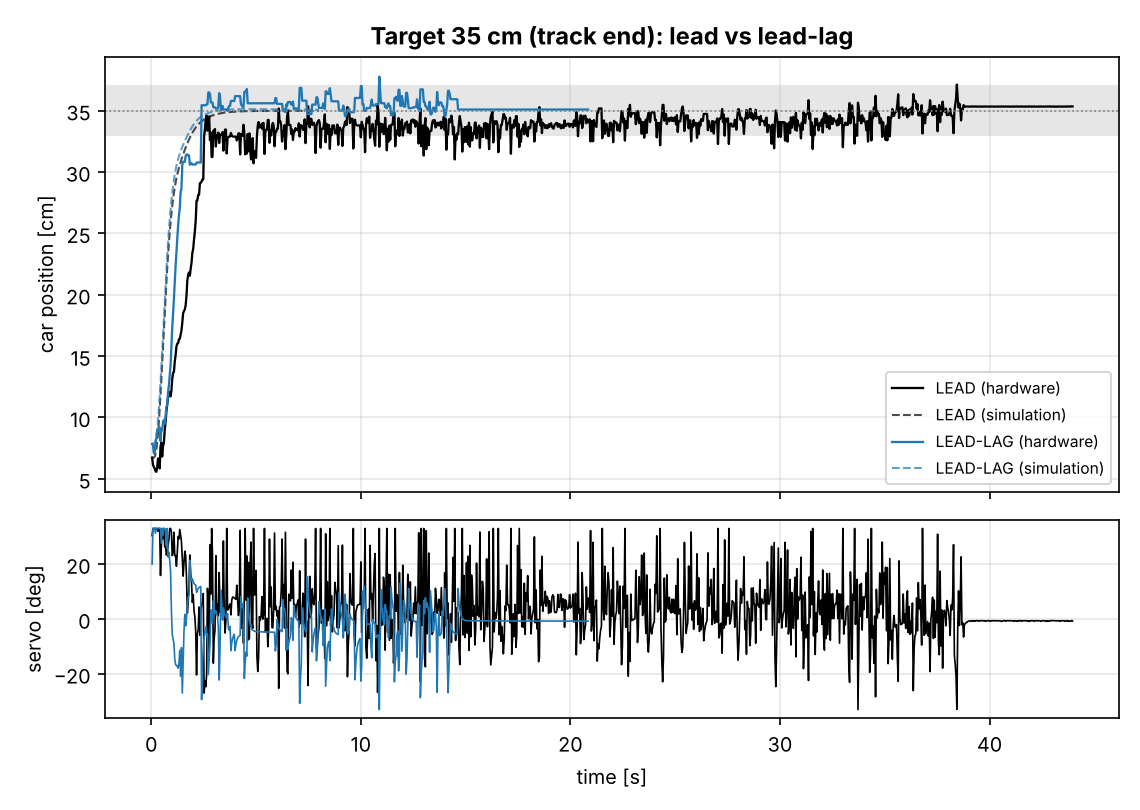
\includegraphics[width=0.92\linewidth]{figures/fig18.png}
\caption{Target 35 cm (the far end of the track).}\label{fig:18}
\end{figure}

\textbf{Target 35 cm, lead and lead-lag.}

From Part 1, the car touches the far end of the track at a sensor
reading of about 34.5 cm, so a 35 cm target is at or just past the end
stop. Both controllers reached the end region in about 2.5 s (rise times
1.84 s and 1.68 s). With the lead the readings near the end jumped by 1
to 3 cm from sample to sample (long range echoes are less reliable, and
the code keeps the last value when an echo is missing, which makes flat
steps). The lead multiplies fast changes by its high frequency gain Kc/α
= 19.7 deg/cm, so a 1.5 cm reading jump becomes a 30 deg servo jump.
That is why the servo chattered between its two limits for about 35 s
while the car shuffled between 31.5 and 35 cm. It finally rested against
the end at 35.33 cm. The lead-lag run had the same noisy readings
(single spikes up to 37.8 cm are echo errors, not real motion) but
settled within 14 s at 35.09 cm.

\hypertarget{simulation-against-hardware}{%
\subsection{Simulation against
hardware}\label{simulation-against-hardware}}

\begin{itemize}
\tightlist
\item
  During the motion the hardware follows the simulation well: rise times
  of 1.1 to 1.8 s against 1.3 s simulated, and little or no overshoot on
  the approach (0 to 1.1 \%). The identified model and the lead design
  are therefore correct for the moving car.
\item
  The hardware is slightly slower at the start of large moves because
  the servo sits at its ±30 deg limit for the first 0.5 to 1 s, and the
  car must first break static friction. The linear simulation has
  neither effect.
\item
  The big difference is the final position. The lead leaves an offset of
  1.7 to 4.8 cm wherever its command Kc x e falls inside the friction
  band. The linear model cannot predict this; it is the same dead band
  effect found in Part 1.
\item
  The lead-lag removes the offset (0.09 to 0.43 cm final error) because
  its low frequency gain is 10 times higher and grows slowly with time,
  so any remaining error eventually produces enough servo angle to move
  the car.
\end{itemize}

\hypertarget{response-to-the-hand-pushes-perturbations}{%
\subsection{Response to the hand pushes
(perturbations)}\label{response-to-the-hand-pushes-perturbations}}

The pushes were given to free the car when friction held it, but they
are also clean perturbations: the car was suddenly displaced and the
controller had to bring it back.

\begin{itemize}
\tightlist
\item
  Lead-lag, target 10 cm, push at 29.9 s: the car was pushed 4 cm past
  the target and was back within ±1 cm 1.1 s later, with no further
  oscillation.
\item
  Lead-lag, target 22.12 cm, push at 15.9 s: the car was pushed 10 cm
  away, overshot by 2.1 cm on the way back and was within ±2 cm 2.1 s
  after the push.
\item
  Lead-lag, target 10 cm, push at 23.3 s: pushed 10 cm away, pulled back
  to within 3 cm in about 1 s, then held by friction again until the
  second push.
\end{itemize}

In every case the loop stayed stable and returned the car to the target,
which is the behaviour Task 8 asks to demonstrate.

\hypertarget{limitations}{%
\subsection{Limitations}\label{limitations}}

\begin{itemize}
\tightlist
\item
  Friction: the dead band of roughly ±8 to 12 deg of servo is the main
  source of error with the lead. At some spots on the track it held the
  car even against larger commands, and a push by hand was needed to
  free it.
\item
  Sensor noise: the HC-SR04 is noisy at long range and gives occasional
  ghost readings, which the lead amplifies into servo chatter near the
  far end.
\item
  Saturation and delay: the ±30 deg servo limit slows large moves, and
  the stored lag command adds overshoot after the car has been stuck.
\item
  Possible improvements: an anti-windup rule that freezes the lag stage
  while the car is stuck, a median filter on the sensor, and targets
  kept at least 2 cm away from the track ends.
\end{itemize}

\hypertarget{conclusions}{%
\section{Conclusions}\label{conclusions}}

\begin{itemize}
\tightlist
\item
  Four chirp experiments, cleaned and analysed in MATLAB, gave the
  transfer function G(s) = 2.591/(s² + 0.4789 s + 0.002551) cm/deg with
  a 60.6 \% fit. Unconstrained n4sid fitted noise; imposing the physical
  structure (two poles, no zero) gave a model close to the Part 1 double
  integrator with 76 \% of its gain, a slow drag pole, and about 0.1 s
  of delay seen in the measured phase.
\item
  Root locus, Nyquist and Bode agree that the uncompensated loop is
  stable but poorly damped: phase margin 16.9 deg (8.8 deg with delay),
  62 \% overshoot and 12 s settling. A gain alone cannot fix it.
\item
  A lead compensator (ωc = 4 rad/s, α = 0.1, Kc = 1.966) with a
  prefilter raises the phase margin to 61.7 deg (41.1 deg with delay)
  and gives 0 \% overshoot with 2.1 s settling in simulation. A lag
  alone fails the specifications; a lead-lag meets them with 10 times
  more low frequency gain.
\item
  On the hardware the lead moved the car to the target region in about
  1.5 to 2 s, matching the simulation, but friction left a 1.7 to 4.8 cm
  offset. The lead-lag removed that offset (0.09 to 0.43 cm). Where
  friction held the car a light push by hand freed it, and the loop
  returned the car to the target within 1 to 2 s, so the lead-lag is the
  best controller for this setup.
\end{itemize}

\hypertarget{matlab-script-es245_part2_solve.m-main-steps}{%
\appendix
\section{MATLAB script (ES245\_Part2\_Solve.m), main
steps}\label{matlab-script-es245_part2_solve.m-main-steps}}

\begin{lstlisting}
% Task 5a: load each log, drop t < 10 s and -1 readings, fix spikes, resample
tok = regexp(fileread(file), '(\d+),(-?[\d\.]+),(-?[\d\.]+)', 'tokens');
M   = str2double(vertcat(tok{:}));            % time_ms, servo_deg, dist_cm
keep = (t >= 10) & (y > 0);
med = movmedian(y,7); bad = abs(y-med) > 2.5; y(bad) = med(bad);
data = iddata(y - mean(y), u - 89, 0.02);

% Task 5b: n4sid, then structured estimate (2 poles, no zero)
sys_n4 = n4sid(dEst, 2, 'Ts', 0, n4sidOptions('Focus','simulation'));
sys_id = tfest(dEst, idtf(3,[1 0.5 0.5]), tfestOptions('InitialCondition','estimate'));
G = tf(sys_id);  compare(dEst, sys_n4, sys_id);  bode(G)

% Task 6
rlocus(G); nyquist(G); margin(G); allmargin(G*exp(-0.09*s))
step(feedback(G,1)); stepinfo(feedback(G,1),'SettlingTimeThreshold',0.05)

% Task 7: lead design
wc = 4; alpha = 0.1; T = 1/(wc*sqrt(alpha));
C0 = (T*s+1)/(alpha*T*s+1); Kc = 1/abs(freqresp(C0*G, wc)); C = Kc*C0;
F  = 1/(T*s+1);  margin(C*G);  step(F*feedback(C*G*pade(exp(-0.09*s),3),1))
Cd = c2d(C, 0.04, 'tustin')                   % coefficients for the Arduino
\end{lstlisting}

\hypertarget{arduino-control-loop-es245_leadlag_target.ino}{%
\section{Arduino control loop
(ES245\_LeadLag\_Target.ino)}\label{arduino-control-loop-es245_leadlag_target.ino}}

\begin{lstlisting}
// first order section: y[k] = b0*x[k] + b1*x[k-1] + a1*y[k-1], limited to +/-30 deg
Stage lead = {16.0876, -15.2938, 0.596204, 0, 0};
Stage lag2 = {1.003599, -0.995602, 0.999200, 0, 0};
const float F0 = 0.02467, F1 = 0.95065;          // prefilter

// every 40 ms:
pos = 0.7 * readCm() + 0.3 * pos;                 // measure and smooth
rf  = F0 * (target + rPrev) + F1 * rf;            // prefilter the target
rPrev = target;
float e = rf - pos;
float u = (mode == 1) ? lead.run(e)               // LEAD
                      : lag2.run(lead.run(e));    // LEAD-LAG
float err = target - pos;                         // friction kick
if (err >  0.5) u += KICK;
if (err < -0.5) u -= KICK;
servo.write(LEVEL + constrain(u, -30, 30));       // servo limited to +/-30 deg
\end{lstlisting}

\end{document}
